%% LLT: Turn off some annoying warnings...
\RequirePackage{silence}
\WarningFilter{titlesec}{Non standard sectioning command}
\WarningFilter{scrreprt}{Usage of package}
\WarningFilter{scrreprt}{Activating an ugly workaround}

% **************************************************
% Document Class Definition
% **************************************************
\documentclass[%
	paper=A4,					% paper size --> A4 is default in Germany
%	twoside=true,				% onesite or twoside printing
    oneside=true,
	twoside=false,				% onesite or twoside printing
	openright,					% doublepage cleaning ends up right side
	parskip=full,				% spacing value / method for paragraphs
	chapterprefix=true,			% prefix for chapter marks
	11pt,						% font size
	headings=normal,			% size of headings
	listof=totoc,				% include listof entries in toc
	titlepage=on,				% own page for each title page
	captions=tableabove,		% display table captions above the float env
	draft=false,				% value for draft version
]{scrreprt}%


\usepackage{ngerman}
\usepackage{hyperref}
\usepackage{wrapfig}
\usepackage[export]{adjustbox}
\usepackage{mathtools}
\usepackage{tocloft}
\usepackage{acronym}
\usepackage[utf8]{inputenc}		% defines file's character encoding
\usepackage{paralist}          % for compactitem itemization
\usepackage{chngcntr}           % Einfache Nummerierung von Abbildungen
\usepackage{blindtext}
\counterwithout{figure}{chapter} % Einfache Nummerierung von Abbildungen
\usepackage{listings} % Code Listings
\usepackage{xcolor}
\usepackage{subcaption}
\usepackage{gensymb}
\usepackage[utf8]{inputenc}


%=====
\lstset{
	language=Python,
	basicstyle=\ttfamily,
	otherkeywords={self},             
	keywordstyle=\ttfamily\color{blue!90!black},
	keywords=[2]{True,False},
	keywords=[3]{ttk},
	keywordstyle={[2]\ttfamily\color{yellow!80!orange}},
	keywordstyle={[3]\ttfamily\color{red!80!orange}},
	emph={def, return},          
	emphstyle=\ttfamily\color{red!80!black},    
	stringstyle=\color{blue!80!black},
	showstringspaces=false            
}
%======
\usepackage{float} % exaktes Figure Placement mit H
\lstset{
  breaklines=true,
%  numbers=left,
  numbersep=5pt,
  basicstyle=\footnotesize\ttfamily,
 % numberstyle=\tiny\color{black}
%  literate=%
%  {Ö}{{\"O}}1
%  {Ä}{{\"A}}1
%  {Ü}{{\"U}}1
%  {ß}{{\ss}}2
%  {ü}{{\"u}}1
%  {ä}{{\"a}}1
%  {ö}{{\"o}}1
}

\lstset{literate=
  {á}{{\'a}}1 {é}{{\'e}}1 {í}{{\'i}}1 {ó}{{\'o}}1 {ú}{{\'u}}1
  {Á}{{\'A}}1 {É}{{\'E}}1 {Í}{{\'I}}1 {Ó}{{\'O}}1 {Ú}{{\'U}}1
  {à}{{\`a}}1 {è}{{\`e}}1 {ì}{{\`i}}1 {ò}{{\`o}}1 {ù}{{\`u}}1
  {À}{{\`A}}1 {È}{{\'E}}1 {Ì}{{\`I}}1 {Ò}{{\`O}}1 {Ù}{{\`U}}1
  {ä}{{\"a}}1 {ë}{{\"e}}1 {ï}{{\"i}}1 {ö}{{\"o}}1 {ü}{{\"u}}1
  {Ä}{{\"A}}1 {Ë}{{\"E}}1 {Ï}{{\"I}}1 {Ö}{{\"O}}1 {Ü}{{\"U}}1
  {â}{{\^a}}1 {ê}{{\^e}}1 {î}{{\^i}}1 {ô}{{\^o}}1 {û}{{\^u}}1
  {Â}{{\^A}}1 {Ê}{{\^E}}1 {Î}{{\^I}}1 {Ô}{{\^O}}1 {Û}{{\^U}}1
  {œ}{{\oe}}1 {Œ}{{\OE}}1 {æ}{{\ae}}1 {Æ}{{\AE}}1 {ß}{{\ss}}1
  {ű}{{\H{u}}}1 {Ű}{{\H{U}}}1 {ő}{{\H{o}}}1 {Ő}{{\H{O}}}1
  {ç}{{\c c}}1 {Ç}{{\c C}}1 {ø}{{\o}}1 {å}{{\r a}}1 {Å}{{\r A}}1
  {€}{{\EUR}}1 {£}{{\pounds}}1
}
\usepackage{color}
\definecolor{javared}{rgb}{0.6,0,0} % for strings
\definecolor{javagreen}{rgb}{0.25,0.5,0.35} % comments
\definecolor{javapurple}{rgb}{0.5,0,0.35} % keywords
\definecolor{javadocblue}{rgb}{0.25,0.35,0.75} % javadoc

% **************************************************
% Debug LaTeX Information
% **************************************************
%\listfiles

% **************************************************
% Information and Commands for Reuse
% **************************************************

\newcommand{\thesisTitle}{\Huge MASTER THESIS}
\newcommand{\thesisTitleEng}{\Large \uppercase{User position prediction in 6-DoF Mixed Reality Applications using Recurrent Neural Networks}}
\newcommand{\thesisName}{Oleksandra Baga}
\newcommand{\thesisDate}{29.06.2022}
%\newcommand{\thesisVersion}{Final}

\newcommand{\thesisFirstReviewer}{Prof. Dr. Daniel Göhring}
\newcommand{\thesisFirstReviewerUniversity}{\protect{Freie Universität Berlin}}
\newcommand{\thesisFirstReviewerDepartment}{Fachbereich Mathematik und Informatik}

\newcommand{\thesisSecondReviewer}{Prof. Dr. Tim Landgraf}
\newcommand{\thesisSecondReviewerUniversity}{\protect{Freie Universität Berlin}}
\newcommand{\thesisSecondReviewerDepartment}{Fachbereich Mathematik und Informatik}


% **************************************************
% Load and Configure Packages
% **************************************************

\usepackage[british,UKenglish,USenglish,english,american]{babel}
%\usepackage[ngerman]{babel} % babel system, adjust the language of the content
\usepackage[					% clean thesis style
	figuresep=colon,%
	sansserif=false,%
	hangfigurecaption=false,%
	hangsection=true,%
	hangsubsection=true,%
	colorize=full,%
	colortheme=bluegreen,%
]{cleanthesis}

\hypersetup{					% setup the hyperref-package options
	pdftitle={\thesisTitle},	% 	- title (PDF meta)
	pdfauthor={\thesisName},	% 	- author (PDF meta)
	plainpages=false,			% 	-
	colorlinks=false,			% 	- colorize links?
	pdfborder={0 0 0},			% 	-
	breaklinks=true,			% 	- allow line break inside links
	bookmarksnumbered=true,		%
	bookmarksopen=true			%
}

% **************************************************
% Document CONTENT
% **************************************************
\usepackage[backend=bibtex,
style=numeric,
maxnames=6
]{biblatex}
\addbibresource{bib-refs.bib}

\begin{document}



% --------------------------
% rename document parts
% --------------------------
%\renewcaptionname{english}{\figurename}{Abb.}
%\renewcaptionname{english}{\tablename}{Tab.}
% -------------------------
% Front matter
% --------------------------
\pagenumbering{roman}			% roman page numbing (invisible for empty page style)
\pagestyle{empty}				% no header or footers
% !TEX root = ../thesis-example.tex
% !TeX spellcheck = de_DE
% ------------------------------------  --> main title page
\begin{titlepage}
	\pdfbookmark[0]{Titlepage}{Titlepage}
	\tgherosfont
	\centering

	
\includegraphics[width=10cm]{gfx/fu_logo} \\[12mm]



%	\textsf{\thesisUniversityGroup} \\
    {\normalsize Freie Universität Berlin}\\
    {\normalsize Fachbereich Mathematik und Informatik}\\
    {\normalsize Takustraße 9, 14195 Berlin}\\[10mm]
	\hspace*{25pt}
	{\LARGE \color{ctcolortitle}\textbf{\thesisTitle}}\\[5mm]
	{\color{ctcolortitle}\textbf{\thesisTitleEng}}\\[40mm]


	
	{\LARGE \thesisName} \\[5mm]
	    {\normalsize Freie Universität Berlin} \\
	    \hspace*{15pt}
    {\normalsize Matrikelnummer 5480722} \\
	{\normalsize Master Computer Science} \\
	\hspace*{50pt}


	{\small E-Mail: oleksandra.baga@gmail.com} \\
	\hspace*{200pt}

	\vfill
	
	\hspace*{15pt}
	\begin{minipage}[t]{.65\textwidth}
		\centering
		{\large \thesisFirstReviewer} \\
	  	{\small \thesisFirstReviewerDepartment} \\[-1mm]
		{\small \thesisFirstReviewerUniversity}
			\hspace*{15pt}
	\end{minipage} \\[15mm]

\hspace*{15pt}
\begin{minipage}[t]{.65\textwidth}
	\centering
	{\large \thesisSecondReviewer} \\
	{\small \thesisSecondReviewerDepartment} \\[-1mm]
	{\small \thesisSecondReviewerUniversity}
	
\end{minipage} \\[5mm]

\end{titlepage}		% INCLUDE: all titlepages
\cleardoublepage

\setcounter{tocdepth}{4}		% define depth of toc
%\setcounter{secnumdepth}{4}
\clearpage

% !TeX spellcheck = en_EN 
\chapter*{Statutory Declaration}
I herewith formally declare that I have written the submitted master thesis independently. I did not use any outside support except for the quoted literature and other sources mentioned in the paper. 

I clearly marked and separately listed all of the literature and all of the other sources which I employed when producing this academic work, either literally or in content. 


I am aware that the violation of this regulation will lead to failure of the thesis.\\\\\\

29.06.2022........................................................................................ Oleksandra Baga


% !TeX spellcheck = en_EN 
\chapter*{Acknowledgments}
This thesis was created in cooperation with the Fraunhofer Heinrich Hertz Institute.

First and foremost I would like to thank Prof FU Berlin, who supervised my thesis. Thank you very much for the helpful suggestions and constructive criticism.

A special thanks goes to the researcher Fraunhofer Heinrich Hertz Institute, Serhan Gül, who suggested an exciting topic for a research, which I was allowed to choose for my master thesis. I would like to express my sincere thanks for the commitment and the consultation during the preparation of this thesis.


\clearpage
\tableofcontents				% display table of contents
\cleardoublepage

% --------------------------
% Body matter
% --------------------------
\pagenumbering{arabic}			% arabic page numbering
\setcounter{page}{1}			% set page counter

\pagestyle{maincontentstyle} 	% fancy header and footer

\pagenumbering{Roman}
\setcounter{page}{1}
% !TeX spellcheck = en_EN
\chapter*{List of Figures}
\label{sec:list_img}
%\addcontentsline{toc}{chapter}{\protect\numberline{}Abbildungsverzeichnis}%
\addcontentsline{toc}{chapter}{List of Figures}%
\renewcommand{\cftfigpresnum}{Fig. } 
\renewcommand{\listfigurename}{}
\setlength{\cftfignumwidth}{2 cm}
\listoffigures{}% Abbildungsverzeichnis

%================================
\lstlistoflistings
%================================
\chapter*{List of Abbreviations}
\label{sec:list_abbr}
\addcontentsline{toc}{chapter}{List of Abbreviations}%
\begin{acronym}[SEPSEPSSEP]\itemsep=-15pt
	\acro{AR}{Augmented Reality}
	\acro{CNN}{Convolutional Neural Network}
	\acro{CPU}{Central processing unit }
	\acro{DoF}{Degree of freedome}
	\acro{DL}{Deep Learning}
	\acro{KF}{Kalman Filter}
	\acro{GRU}{Gated Recurrent Unit}
	\acro{HMD}{Head-Mounted-Display}
	\acro{IEEE}{Institute of Electrical and Electronics Engineers}
	\acro{ISO}{International Organization for Standardization}
	\acro{LAT}{Look ahead time}
	\acro{LSTM}{Long-Short-Term Memory}
	\acro{M2P}{Motion-to-Photon}
	\acro{MAE}{Mean Absolut Error}
	\acro{MEC}{Mobile Edge Computing}
	\acro{ML}{Machine Learning}
	\acro{MR}{Mixed Reality}
	\acro{NLP}{Natural Language Processing}
	\acro{ReLu}{Rectified Linear Unit}
	\acro{RNN}{Recurrent Neural Network}
	\acro{SDG}{Stochastic Gradient Descent}
	\acro{VR}{Virtual Reality}
	\acro{3-DoF}{Three degree of freedome}
	\acro{6-DoF}{Six degree of freedome}
\end{acronym}

\clearpage
\pagenumbering{arabic}
\setcounter{page}{1}





% !TeX spellcheck = en_EN
\chapter{Introduction}
\label{sec:intro}
This thesis is focusing on designing and evaluation of the new approach for the predicting human head motion with a 6-dimensional degree of freedom (DoF) for Extended Reality (XR) applications. 


\section{Problem statement}
\label{sec:intro:problem}
A non-full-text database that typically contains article metadata, abstracts, and subject classifications. Used by researchers to locate publications relevant to their research

\section{Motivation for the research}
\label{sec:intro:motivation}
The following chapter introduces the preprocessing pipeline, architecture, and evaluation process used to develop ahead motion prediction algorithm.


\section{Structure of the thesis}
\label{sec:intro:structure}
The organization of this thesis is as follows. The literature review chapter introduces the concepts of XR technologies and principles of motion prediction algorithms. It follows an overview of previous research. 

\textbf{Chapter 1} - Introduction.\\
The following chapter introduces the preprocessing pipeline, architecture, and evaluation process used to develop ahead motion prediction algorithm.





% !TeX spellcheck = en

\chapter{Fundamentals}
\label{sec:theorie}
This chapter introduces theoretical background of the presented research problem. First, the concept of mixed reality (MR) followed by an introduction of six degree of freedom (6-DoF) environment and the difference to the three degree of freedom (3-DoF) are described. The term motion-to-photon latency (M2P) is covered, followed by a short discussion about an influence of M2P latency on the decreasing of user experience. The new developed cloud-based rendering and streaming approach is shortly discussed in this chapter. The last section of this chapter highlights challenges with the prediction of viewer's head pose that arises in modern XR applications in connection especially with the added network latency due the using of remote cloud server for computational offload. The section \ref{sec:related} overviews the existing works done in the research field using traditional algorithms and recurrent neural networks. 
%##############################################
\section{Mixed reality with HMD}
\label{sec:theorie:ar}
Mixed reality makes possible to break down the border between the virtual and real world and provides today an experience that just a short-time ago we could only imagine when watching the sci-fi movies. Terms Virtual Reality (VR), Augmented reality (AR) and Mixed reality (MR) are often used interchangeably. VR creates the virtual environment around user and tricks human's senses into thinking one is in a different environment. AR adds a virtual object to the real world that we can see through the lenses of special developed Head Mounted Display (HMD). Thus realistic images, sounds, and other sensations can be generated by a powerful HMD and projected on transparent holographic lenses giving a user the feeling that virtual objects have size and density. However, AR does not allow interactions between users and the virtual objects added to the real-world scene. MR combines the advantages of the VR and AR and adds an interaction between real and artificial elements. Thus users can directly interact with virtual objects (with operations such as scaling, rotation, or translation) in the real environment using their hands. For example, in MR Application virtual objects can be placed on the real table in the user's room, picked up with a hand and moved to another place.\\
%##############################################
Volumetric video (VV) is a new content creation approach to be used within AR and MR applications \cite{user_behav_volumetric}. Volumetric video allows to view recorded information from a range of different angles, as if an observer was physically presented in the room when video was captured by cameras and could move around the object. This thesis uses volumetric video object placed in the real environment when running developed MR Application for collection the user's position and rotation data. Refer sections \ref{sec:theorie:cloud} and \ref{sec:impl:model:dev:unity} for more details about VV and how it was used in thesis. 
%############################################
\begin{wrapfigure}{L}{0.5\textwidth}
	\centering
	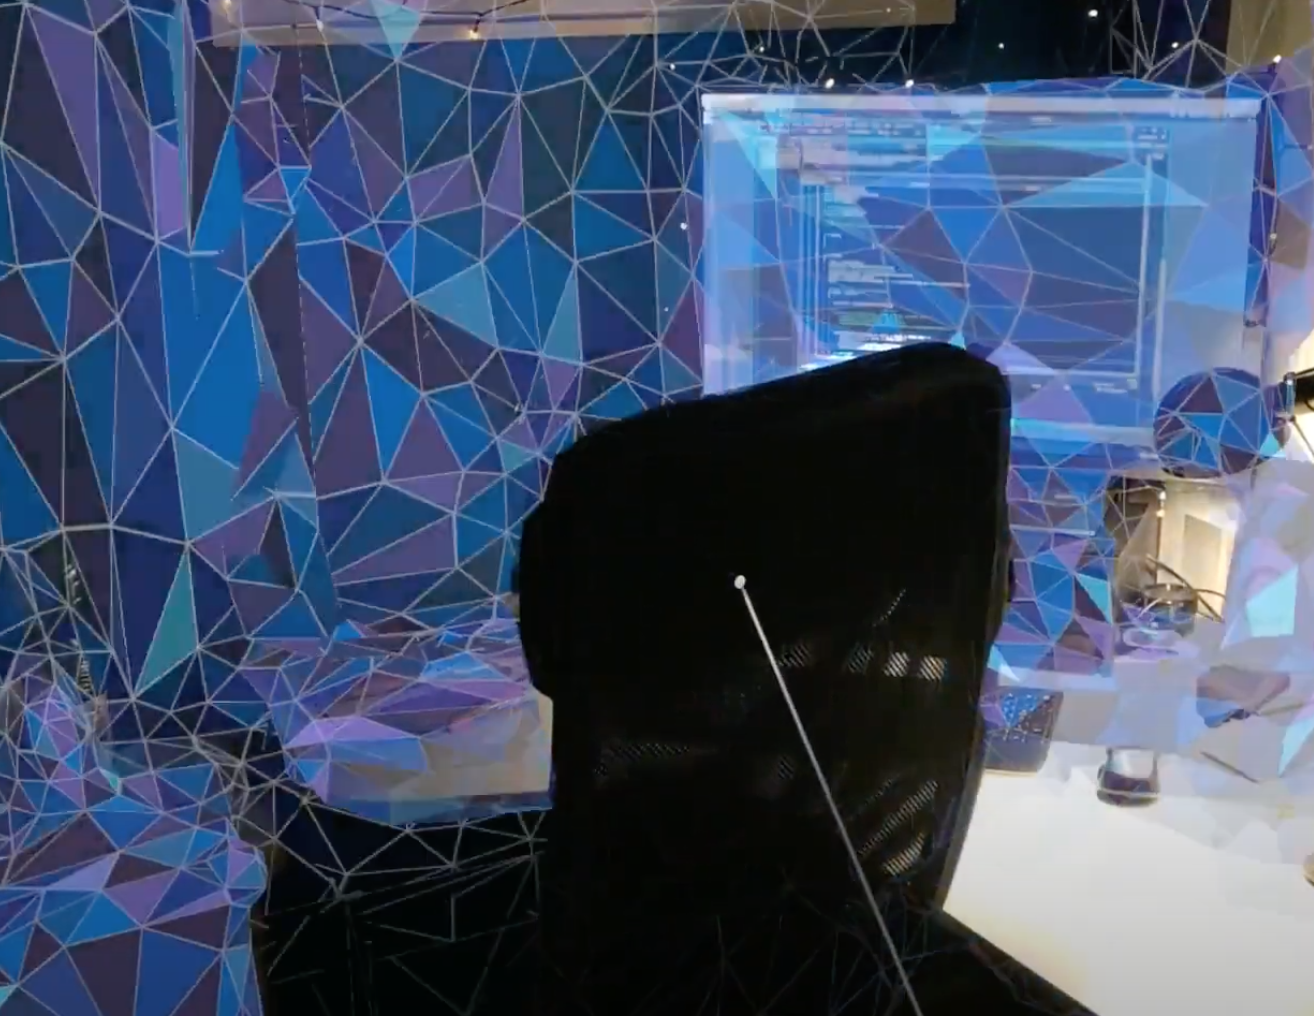
\includegraphics[width=0.47\textwidth]{gfx/hololens_env.png}
	\caption{\label{fig:holo2_env}HoloLens 2 maps itself with a mesh.}
\end{wrapfigure}

Nowadays different HMD with varying performance levels and prices are available on the market. In this thesis, Microsoft HoloLens 2 was used for MR experience and data collection. It is an updated version of the previous generation HoloLens 1 headset from Microsoft with such improved feature as display resolution, field of view, weight, battery lifetime. By using the AHAT (Articulated HAnd Tracking) depth camera, the HoloLens 2 can capture hand movements to obtain hand tracking data. The build-in tracking systems allows HoloLens to understand the environment around the user and to place stable and accurate holograms on the correct places where they intended to be by the developer of MR Application. The data used to track users is represented in the spatial map\footcite{https://docs.microsoft.com/en-us/hololens/hololens-environment-considerations}. When VR Application is starting on HoloLens, HoloLens uses unique environmental landmarks to locate itself in a space. The mesh graphic spreading over the space is seen, as illustrated in Fig. \ref{fig:holo2_env}, during the Application launch and this means a device is mapping to surroundings. As user moves with HMD on their head, built-in cameras continuously scan the environment and construct virtual world geometry for real-world objects. The primary stereo rendering component attached to HMD can be accessed from Unity and thus the position and orientation can obtained for thesis purposes. 

%##############################################
\section{Six degrees of freedom}
\label{sec:theorie:6dof} 
Term \textit{degrees of freedom} describes how users interact with a virtual environment and how they can move inside it. Within 3-DoF space user has only three possibilities: look left and right, look up and down and pivot left and right. 3-DoF space does not allow to move throughout the virtual space. Thus only rotational movement can be tracked. In 3-DoF VR Application multimedia content is the omnidirectional or spherical video, which represents an entire 360$^{\circ}$ environment on a virtual sphere \cite{6-dof_metrics}. In 3-DoF space HMD enables to display only a portion of the environment around a user. User is virtually positioned at the centre of a sphere as shown in Fig. \ref{fig:3and6dof}, media is displayed from an inward position and user can only change the viewing direction (i.e., by looking up/down or left/right or tilting the head side to side) \cite{6-dof_metrics} but can not interact with a media by moving closer/further. Wherever user moves with a HMD on their head, they will remain placed in the  at the centre of a sphere and distance to a content can not be changed.
\begin{wrapfigure}{R}{0.4\textwidth}
	\centering
	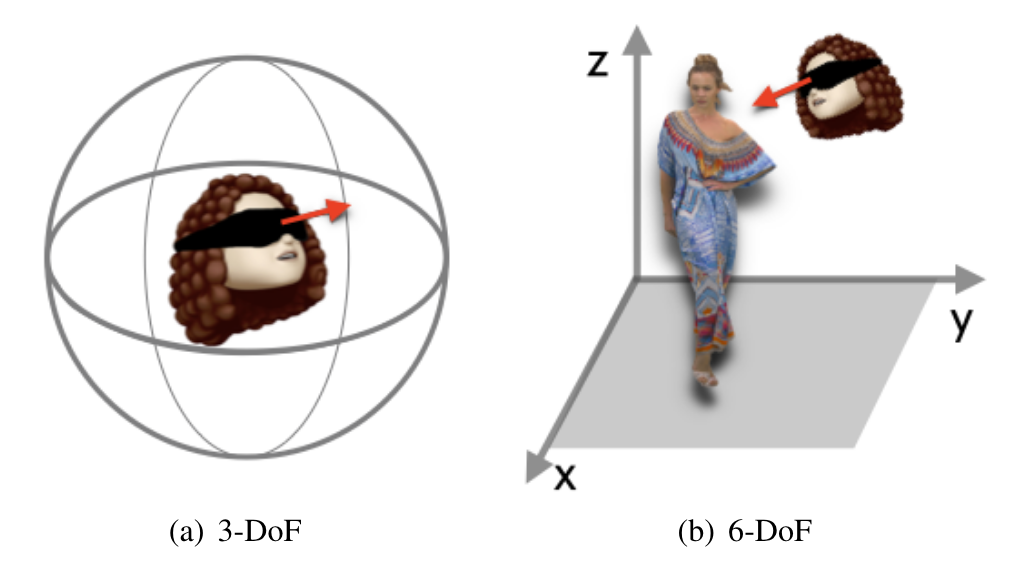
\includegraphics[width=0.37\textwidth]{gfx/3-6dof.png}
	\caption{\label{fig:3and6dof}Viewing paradigm in 3- and 6-DoF VR. Source: \cite{6-dof_metrics}}
\end{wrapfigure}

The new VR concept 6-DoF means tracking both position and rotation and refers to the freedom of movement of a rigid body in three-dimensional space. In 6-DoF VR Application user can also change viewing perspective by moving (e.g., walking, jumping) inside the virtual space \cite{6-dof_metrics}. Thus the scene is observed from an outward position in 6-DoF environment and extra degree of freedom transforms the virtual experience to be more natural and reflects to human movement in a three-dimensional space. Thus the VV and other volumetric objects such meshes or point clouds are used in MR Applications for 6-DoF scene population. User can freely walks inside the 6-DoF environment with a HMD on a head and observe the placed on scene volumetric objects from all points of view, and if the settings in Unity application allow physical interaction with objects, pick and move them on the new place. 

\section{Motion-to-photon latency}
\label{sec:theorie:m2p}
VR Application are deployed to the end-user with a goal to create an immersion of a physical presence in a non-physical world. In the real world there is no time delay between action taken and reaction observed. However, in AR/VR/MR Applications the difference between the user's head movement (action) and its corresponding display output reflections (reaction) is defined as motion-to-photon (M2P) latency. The presence of a delay between the physical movement and the display output worsens HMD user experience. In worst case even sense of physical presence in a virtual world would be lost. MTP latencies of more than 20 ms are experienced and cause spatial disorientation and dizziness, referred to as VR sickness or motion sickness \cite{delay_sickness, serhan_kalman}. Display lag can produce a range of other perceptual effects include degraded vision, compromised visuo-motor performance and motion sickness \cite{delay_sickness}. Different components of the HMD, such as the sensors, SOC, display and software can affect M2P latency. Reducing the M2P latency is the key to proving the best VR experience. Not only improving the device parameters, such a usage of more powerful HMD processor, need to be taken in account. VR Application developers must consider how to deploy more light-weighted applications. If the VR Application need to pull some data from the network or remote server, the network round-trip time and the added processing delays will increase the M2P latency compared to a system that only performs the processing locally \cite{serhan_kalman}.\\

\begin{wrapfigure}{L}{0.48\textwidth}
	\centering
	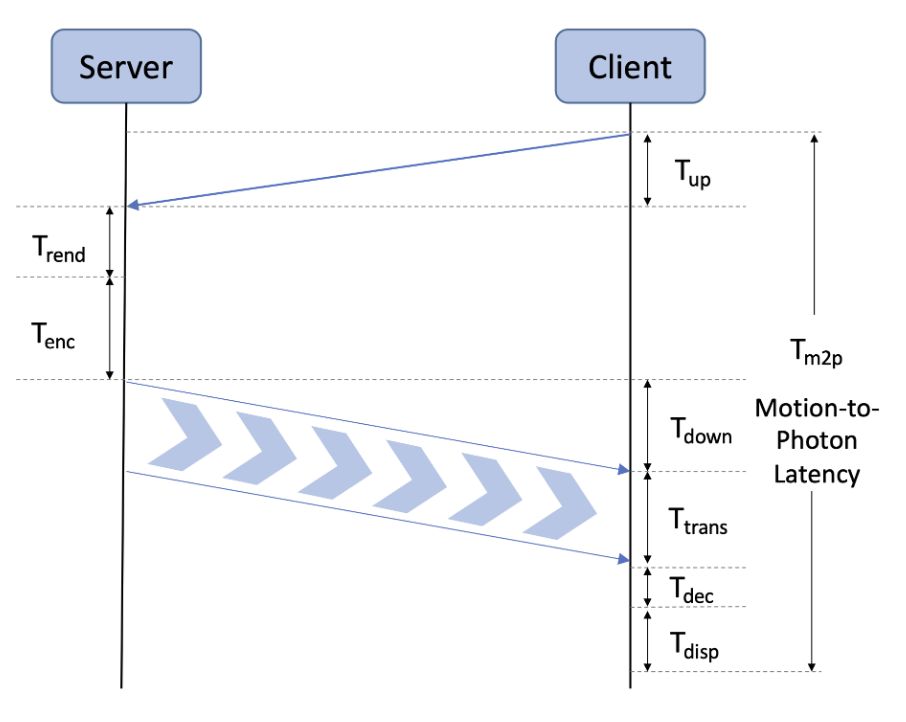
\includegraphics[width=0.46\textwidth]{gfx/m2p.png}
	\caption{\label{fig:m2p}M2P latency for a remote rendering system. Source: \cite{serhan_cloud_streaming}}
\end{wrapfigure}

As this thesis evaluates the reducing the M2P latency for VV streaming from remote cloud server, the Fig. \ref{fig:m2p} illustrates the different components of the M2P latency for a remote rendering system. Total M2P latency is equal to sum of the time taken by a bit of data to travel across the network from HMD to a server, server delay involved in computing the future user position and render a 2D view and a HMD delay during sensor measurements. If the user’s future head pose for a look-ahead time (LAT) equal to or larger than the M2P latency of the system could be predicted, it can eliminate M2P latency and improve the quality of the VR Applications. Studies showed that display lags of greater than 40 ms cause errors in tracking and following a target with the head \cite{delay_sickness}. This thesis evaluates the performance of RNN Models for LAT 100 ms that is higher than the measured M2P latency of a cloud-based volumetric streaming system described in the next section. 

\section{Cloud-based volumetric video streaming}
\label{sec:theorie:cloud}
% User Behaviour Analysis of Volumetric Video in Augmented Reality

\section{Challenges of head motion prediction}
\label{sec:theorie:head_pred}
All modern HMD has a position tracker, a device or a system of devices, that is responsible for reporting  the position and orientation of HMD to the computational unit that generates the virtual environment images displayed in the HMD. These images represent the view that a wearer of HMD would have seen if user was present in VR at the position and orientation reported by position tracker \cite{hmd}.\\
While the task of position tracking is performed by HMD hardware, the task of position prediction of the movement of human body in the virtual reality remains challenging, and it is still complicate to achieve high-precision estimation. Recurrent neural networks have recently shown promising results in many machine learning tasks, especially when input and/or output are of variable length and are coming as time series with a sequential order.  Unfortunately, the known problem of RNN that was observed many years ago by e.g., \textit{Bengio et al., 1994} that it is difficult to train RNNs to capture long-term dependencies because the gradients tend to either vanish (most of the time) or explode (rarely, but with severe effects) \cite{rnn_difficults}. New approaches are needed to be implemented to reduce the negative impacts of this issue. Since traditional recurrent unit overwrites its content at each time-step, a LSTM unit is able to decide whether to keep the existing memory via the introduced gates. The Long Short-Term Memory (LSTM) has a number of minor modifications \cite{empirical_evaluation} since it was initially proposed in work \cite{lstm_orig}. Another approach called a gated recurrent unit (GRU) can adaptively capture dependencies of different time scales without having a separate memory cells \cite{empirical_evaluation}. These two approaches can help to find the long-term dependencies in the data obtained from HMD that are otherwise are hidden by the effect of short-term dependencies from the standard RNN models.\\
%============================================
Not only the NN architecture is important for high prediction accuracy. Understanding how users interact and behave in AR or VR is a key for preparing the correct dataset when working with HMD's sensors. The experiment done by \textit{Zerman et al., 2021} found out that users preferred to stay in front of static point clouds and 1-1.5 meter away from them and spent more time looking at the frontal view and faces of human models \cite{user_behav_volumetric}. The navigation trajectories of users within a 6-Degrees-of-Freedom (DoF) should be additionally investigated. An extra level of interaction between user and content is available in 6-DoF environment. The user has now the freedom to change the viewing direction (rotating and translating the head as in 3DoF) but also to change position inside the VR environment \cite{new_challenge}. In a 3-DoF environment, users are viewing a portion of the omnidirectional content all the time being positioned at the centre of the spherical content. Thus it is important to understand that a distance between user and content is constant during the interaction \cite{new_challenge}. In a 6-DoF, however, the distance changes over time when user moves due to the added degrees of freedom. Thus viewport’s center position is not sufficient for tracking the trajectories, the additional metrics such the spatial coordinates and user orientation are needed to obtain the point of origin. Following \cite{new_challenge} \textit{Rossi et al, 2021} authored same year another work \cite{6-dof_metrics} dedicated 6-DoF metrics. Researchers proposed to change the video detailing based on user distance to the volumetric object. The closer users are to the volumetric content, the smaller and more detailed is the portion of the displayed content; the farther they are, the bigger but with fewer details becomes the displayed portion \cite{6-dof_metrics}. \textit{Rossi et al, 2021} experimented with different metrics to perform clustering in order to detect group of users with similar behavior in VR. The most promising metric seems to be based on the user position on the virtual floor. Metrics based only on viewport center and distance failed in detecting the group of users, which in the ground-truth case form their own cluster, as similar and divided them instead in different clusters \cite{6-dof_metrics}. For the trajectory detection best performed a metrics based on user position on the virtual floor, distance and viewport center. Thus not only the way in which users interact within a 3- and 6-DoF environment is fundamentally different. New physical settings and locomotion functionalities given to users also prevent a straightforward extension of current 3-DoF algorithms to 6-DoF \cite{6-dof_metrics}. The analysis above leads to the conclusions that prediction of the user's position and orientation on 6-DoF not only a contemporary but also a challenging task that requires new metrics and approaches to be investigated and implemented. 
% !TeX spellcheck = en
\section{Related works}
\label{sec:related}
This section presents the overview of previous research in the field of the prediction of user position and focuses on time series methods using different RNN architectures such as LSTM and GRU.  


\subsection{Traditional prediction algorithms}
\label{sec:related:timeseries}
A lot of previous approaches uses basic processing of head movement history to predict the future movement, such as simple average, linear regression, and weighted linear regression \cite{attention_saliency}. Work of \textit{Corbillon et al., 2017} determines the distance to the center of viewpoint with simple average and calculates the region that receives from server the video data with a better quality than the remaining of part the video \cite{simple_average}.\\ The work of \textit{Duanmu et al., 2017} proposes prediction of the viewing direction for segment n + 1 through linear regression based on the past view segments \cite{linreg1}. Approach of \textit{Xie et al., 2017} uses user’s orientation in Euler angle and leverage Linear Regression model to apply Least Square Method and to calculate the trends of head movements \cite{linreg2}. The work \cite{linreg3} proposes to receive from a server only the data of covered by user's viewport. At each point of time, the client requests data which would be played in the future. \textit{Taghavi et al., 2017} use Weighted Linear Regression to predict the next viewport based on window with the latest viewport samples. Researchers mentioned that a client can continue playback of at least a low-quality version of the video when the download time of next video portion varies \cite{linreg3}.\\
Analysis done by \textit{Qian et al., 2016} indicates that at least in the short term, viewers’ head movement can be predicted with accuracy > 90\% by even using simple methods such as linear regression \cite{cellular_opt}. The different approaches were compared such as computing the average value, using the linear regression with all samples and with weighted linear regression with recent samples. With weighted linear regression the average prediction accuracy for short-term values was higher than 90\% across all users. However in the longer term it is more difficult to achieve the good result and the average accuracy drops to about 70\% \cite{cellular_opt}.\\
A method to apply saliency algorithms to VR video viewings was presented by \textit{Aladagli et al., 2017} in work \cite{predicting_360}. Cross-correlation analysis used for measuring the relationship between the predicted fixation sequences and the recorded head movements \cite{predicting_360}. Based on works mentioned above, \textit{Nguyen et al., 2018} proposed panoramic saliency algorithm in order to learn the dependence of head tracking logs and saliency maps from the past video frames.\\

\subsection{Recurrent Neuronal Networks}
\label{sec:related:deep}
As was explained above, traditional prediction algorithms can not be used straightforward on a new media content in 6-DoF VR Applications. The user position and rotation data is coming as time series with a sequential order that is crucial to be followed in order to predict correctly the next future step for a look-ahead time. A sequence of inputs can be processed with Artificial Neural Network (ANN) called Recurrent Neural Network (RNN). Moreover, RNN can processes input with remembering its state while processing the next sequence of inputs. It is known that standard RNN has difficulties to learn long-term dependencies with gradient descent \cite{rnn_difficults}. Though RNN can robustly store information, it yields a problem of vanishing gradient that make leaning difficult \cite{rnn_difficults}. In the last decade, RNN algorithms have been adopted for motion prediction of 3D sequences with long-term dependencies taken into account. For example, the work of \textit{Crivellari et al., 2020} targets traces of tourists in a foreign country and tries to predict the motion of people in the environment they never seen before. LSTM-based model is used thus for analyzing the tourists’ mobility patterns \cite{tourist_traces}.\\
%================================================
The authors \textit{Aykut et al., 2018} claims their research to be first work that applies deep learning for head motion prediction. The authors experimentally confirmed that Feed-forward Neural Network (FFN) indeed had difficulties to learn for different delays. The decision to use LSTM-based architectures \textit{Aykut et al., 2018} reasoned with feedback loop and ability to establish a way of memory and share weights over time \cite{delay_compensation_360}. Conducted by researchers experiments showed that the LSTM-based architecture leads to a significant improvement of the MAE and RMSE metrics \cite{delay_compensation_360}. The LSTM-based methods were compared also to widely used approaches like the Linear Regression and a Kalman Filter based optimal state estimate. Thus \textit{Aykut et al., 2018} demonstrated a substantial improvement of the deep predictor for latencies in the range of 0.1–0.9 s \cite{delay_compensation_360}.\\
%================================================
Next year \textit{Aykut et al., 2019} experimented in their work \cite{telepresence} with GRU model that belongs to the group of recurrent neural networks (RNN). Authors considered GRU usage because it is computationally more efficient, as it has fewer parameters and states than LSTM units \cite{telepresence}. Proposed in the research GRU-based network is able to improve the MAE and RMSE compared to mentioned above LSTM model, especially for larger delays \cite{telepresence}. \\
%================================================
Researchers \textit{Karim et al., 2018} developed long short term memory fully convolutional network (LSTM-FCN). In the proposed models, LSTM block is augmented by an fully convolutional block \cite{lstm_fcn} identical to the convolution block in the CNN architecture proposed by \textit{Wang et al., 2018} in their work \cite{timeseries_scratch}. \textit{Karim et al., 2018} tried to reduce the rapid model's overfitting by transformation of input to have N variables with a single time step \cite{lstm_fcn}.\\
%================================================
In work of \textit{Chang et al., 2020} used in addition to standard LSTM networks also bidirectional LSTM (Bi-LSTM) networks, which is stacked two LSTM networks in forward and backward directions. Standard LSTM networks can only consider the past information and Bi-LSTM networks can capture both past and future information by two opposite temporal order in hidden layers \cite{6DoF_Tracking}. Experimentally, authors found that the basic LSTM performs the best comparing to Bi-LSTM and Temporal Convolutional Network  \cite{6DoF_Tracking}.\\
%================================================
The paper \cite{action_recognition} also aims for action recognition using sensor signals from HMD. Researches used GRU Model and additionally a bidirectional LSTM (Bi-LSTM) network.  Authors mentioned a representation of a signal data by the latent vector in the low-dimensional space after using the CAE model. The latent vector then will be clustered by K-Means Clustering so that centroids are referred to as motion bases in a model. For action tracking with LSTM, the displacement in each timestamp was predicted first and then added to its previous location, instead of predicting each position directly \cite{action_recognition}. Similar as in work \cite{6DoF_Tracking} the 3-layered LSTM model performed better compared to Bi-LSTM. Authors said that the possible reason could be the short-term correlation of human actions in their dataset and that Bi-LSTM with its complicated model structure is rather suitable for long-term actions \cite{action_recognition}.\\
%================================================
The paper of \textit{Chung et al., 2014} should be noted separately in the end of related works review because it provides an interesting compassion and evaluation of the performance of recurrent units LSTM and GRU on sequence modeling. Authors mentioned the ability of LSTM to keep the existing memory via the introduced gates and thus to detect an important feature from an input sequence at early stage, to easily carry this information (the existence of the feature) over a long distance, hence, capturing potential long-distance dependencies \cite{empirical_evaluation}. The GRU takes linear sum between the existing state and the newly computed state similar to the LSTM but does not have any mechanism to control the degree to which its state is exposed, but exposes the whole state each time \cite{empirical_evaluation}. \textit{Chung et al., 2014} emphasize the fact that any important feature, decided by either the forget gate of the LSTM unit or the update gate of the GRU, will not be overwritten but be maintained as it is \cite{empirical_evaluation}. LSTM unit controls the amount of the new memory content and does not have any separate control of the amount of information flowing from the previous time step. The GRU differs and controls the information flow from the previous activation when computing the new and does not independently control the amount of the candidate activation being added via update gate \cite{empirical_evaluation}. The experiments provided in this work clearly indicate the advantages of the gating units over the more traditional recurrent units. \textit{Chung et al., 2014} mentioned that with dataset they used GRU unit outperformed LSTM unit. But they suggest that the choice of the type of gated recurrent unit may depend heavily on the dataset and corresponding task \cite{empirical_evaluation}. Thus in section \ref{sec:design:dataset:explor} of chapter ``Data and Model'' the data exploration of the obtained from HMD Microsoft HoloLend is done in order to understand the dataset before the beginning with a development of model architecture. 
% !TeX spellcheck = en
\chapter{Implementation}
\label{sec:impl}
This chapter presents the steps of development and implementation of the proposed approach. The Unity Application for HoloLens was deployed on HMD and a raw data with measures and dimension columns was obtained. This data than was analysed and preprocessed to ensure that the captured data can be used in corresponding machine learning models. The model architecture was implemented and experimentally improved during training and evaluation steps. 

\section{6-DoF Dataset}
\label{sec:impl:dataset}
This section describes how the dataset was obtained, analysed and presents the visualization of user's head position and rotation. Almost all machine learning approaches require not only row data collection but also data exploration and preprocessing steps to be done before training begins.

\subsection{Data collection from HMD}
\label{sec:impl:dataset:HL}
The real 6-DoF dataset must be used as training data from which the model can learn the spacial and time dependences. In this master thesis HoloLens 2, the second iteration of Microsoft's head-mounted mixed reality device, was used for data collection. The user position and orientation were obtained with Unity application developed for this purpose. Main Camera in Unity is automatically configured to track head movements. More details about Unity application can be found in section \ref{sec:impl:model:dev:unity}. Using the Main Camera, a user position $(x, y, z)$ and orientation in quaternion $(qx, qy, qz, qw)$ were logged in a $csv$-file. Quaternions obtained from HMD will be used to define a rotation by four numbers. Quaternions representations are very convenient for operations such as composition or rotations and coordinate transformation \cite{principles_robot_motion_book}. For these reasons quaternions are chosen for the representation of user head's rotation in three dimensions. Comparing to dataset in \cite{serhan_kalman}, the additional parameters were recorded from the Main Camera in order to add more information during training processes. Thus the world-space speed of the camera in meters per second was recorded. Unity velocity has the speed in $(x, y, z)$ defining the direction. The obtained 6-DoF dataset has 10 features used in training process: position $(x, y, z)$, orientation $(qx, qy, qz, qw)$ and velocity $(x, y, z)$.

The datasets were recorded in the laboratory space. HMD was presented to users and the basic functions were explained. During data recording, users freely walked wearing HMD in laboratory space. The Unity application, running on HMD, not only recorded the mentioned before parameters but also had a volumetric animated object placed 3 meters ahead of the user in the Mixed Reality environment. No personal data was recorded during these sessions and all traces are obtained anonymously. Thus, after an Unity application was launched, user could immediately see the animated object. The several traces were recorded at least for 10 minutes each. It allows to have enough data after splitting the dataset into training, test and validation partitions. Table \ref{tab:raw_data} show the first 20 rows from raw dataset obtained from HoloLens 2 and used in training. Although dataset has 10 columns, the table \ref{tab:raw_data} presents only $timestamp$ and position $(x, y, z)$ columns. 

\begin{table}[!ht]
		\footnotesize
		\centering
	\begin{tabular}{|l|l|l|l|}
		\hline
		timestamp & x & y & z \\ [0.5ex] 
		\hline\hline
		2.649431 & 0.004954389 & 0.003402365 & 0.01010712 \\ \hline
		2.66943 & 0.00459053 & 0.003120769 & 0.01130438 \\ \hline
		2.698009 & 0.003960807 & 0.002990472 & 0.01276976 \\ \hline
		2.719285 & 0.003730714 & 0.003037783 & 0.01305151 \\ \hline
		2.746641 & 0.003252693 & 0.003489003 & 0.01368421 \\ \hline
		2.764094 & 0.003153284 & 0.003518121 & 0.01400959 \\ \hline
		2.780033 & 0.003087142 & 0.003409061 & 0.01435899 \\ \hline
		2.802086 & 0.003021815 & 0.00314023 & 0.01473305 \\ \hline
		2.815575 & 0.002789935 & 0.003551113 & 0.01506916 \\ \hline
		2.832602 & 0.002527435 & 0.003542757 & 0.01534094 \\ \hline
		2.848514 & 0.002212256 & 0.003605011 & 0.01565307 \\ \hline
		2.863769 & 0.001921757 & 0.003369405 & 0.01590317 \\ \hline
		2.879648 & 0.001668522 & 0.00348538 & 0.01607716 \\ \hline
		2.89686 & 0.001501704 & 0.003624826 & 0.01627397 \\ \hline
		2.913541 & 0.001487849 & 0.00359472 & 0.01643924 \\ \hline
		2.930006 & 0.001501501 & 0.003769569 & 0.01669565 \\ \hline
		2.948201 & 0.001617525 & 0.004252479 & 0.01697758 \\ \hline
		2.964302 & 0.001755987 & 0.004224311 & 0.01721937 \\ \hline
		2.97978 & 0.001838901 & 0.004487753 & 0.01747578 \\ \hline
		2.997117 & 0.002005509 & 0.005007531 & 0.01782864 \\ \hline
	\end{tabular}
\caption{\label{tab:raw_data}Raw data from HoloLens 2.}
\end{table}

The first column in dataset is $timestamp$. It is obviously, that timestamp appears in row dataset not linearly and comes with different pauses. Even the high-cost HMD, like used in this research HoloLens 2, is sometimes unstable in frame rate during collecting data. Due to signal processing and propagation delays, distance in time between two consecutive samples was either increased or decreased.
In the Unity Application, the frame rate is 60 Hz which means that data is expected to be collected every 0.016(6) seconds. Data on some expected timestamps seemed to be unavailable in HMS for recording. Between two sequences with bigger time gap, some records may be considered to be missed. To deal with above situation, the preprocessing steps must be done. They are described in a section \ref{sec:impl:dataset:preprocessing} below. 

\subsection{Data Exploration}
\label{sec:impl:dataset:explor} 
The next step after looking at raw data, gathered for machine learning, is a data exploration. The goal of this initial step is, firstly, a data visualization for understanding of dataset characterizations. As already stated in section \ref{sec:impl:dataset:HL}, a user position $(x, y, z)$, orientation in quaternion $(qx, qy, qz, qw)$ and the world-space speed of the camera for each direction in $(x, y, z)$ was obtained from Main Camera in Unity application launched on HMD.\\
\begin{figure}[H]
	\centering
	\begin{subfigure}[b]{1\textwidth}
		\centering
		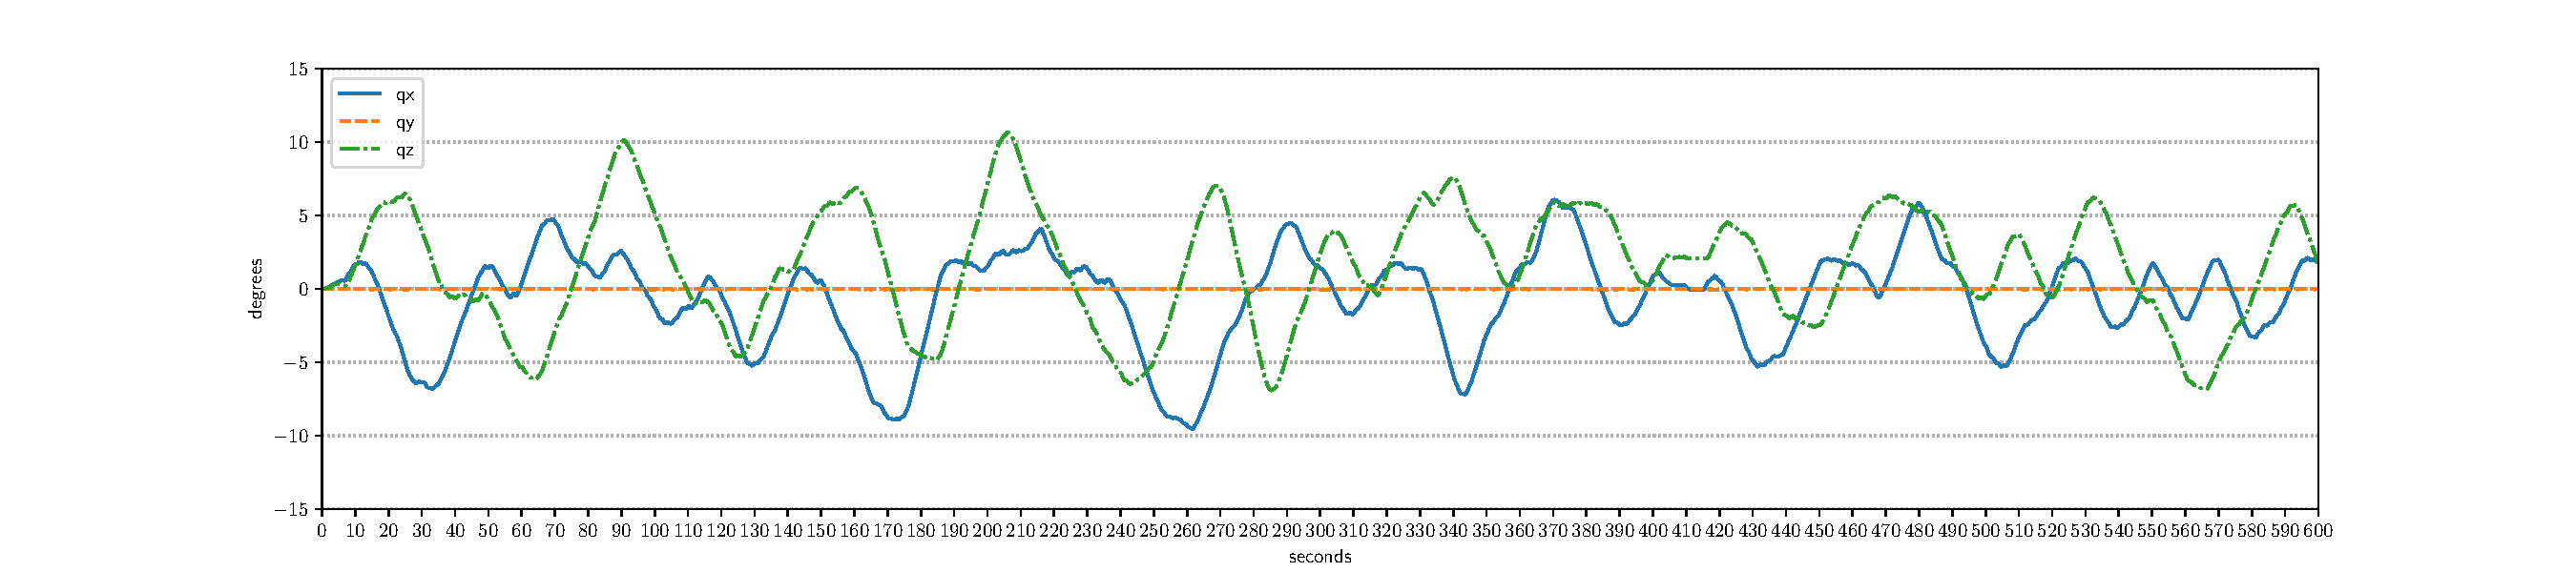
\includegraphics[width=1\textwidth, keepaspectratio]{gfx/Fig-1556-position.pdf}
		\caption{Dataset 1556}
		\label{fig:pos1}
	\end{subfigure}
	\qquad
	\begin{subfigure}[b]{1\textwidth}
		\centering
		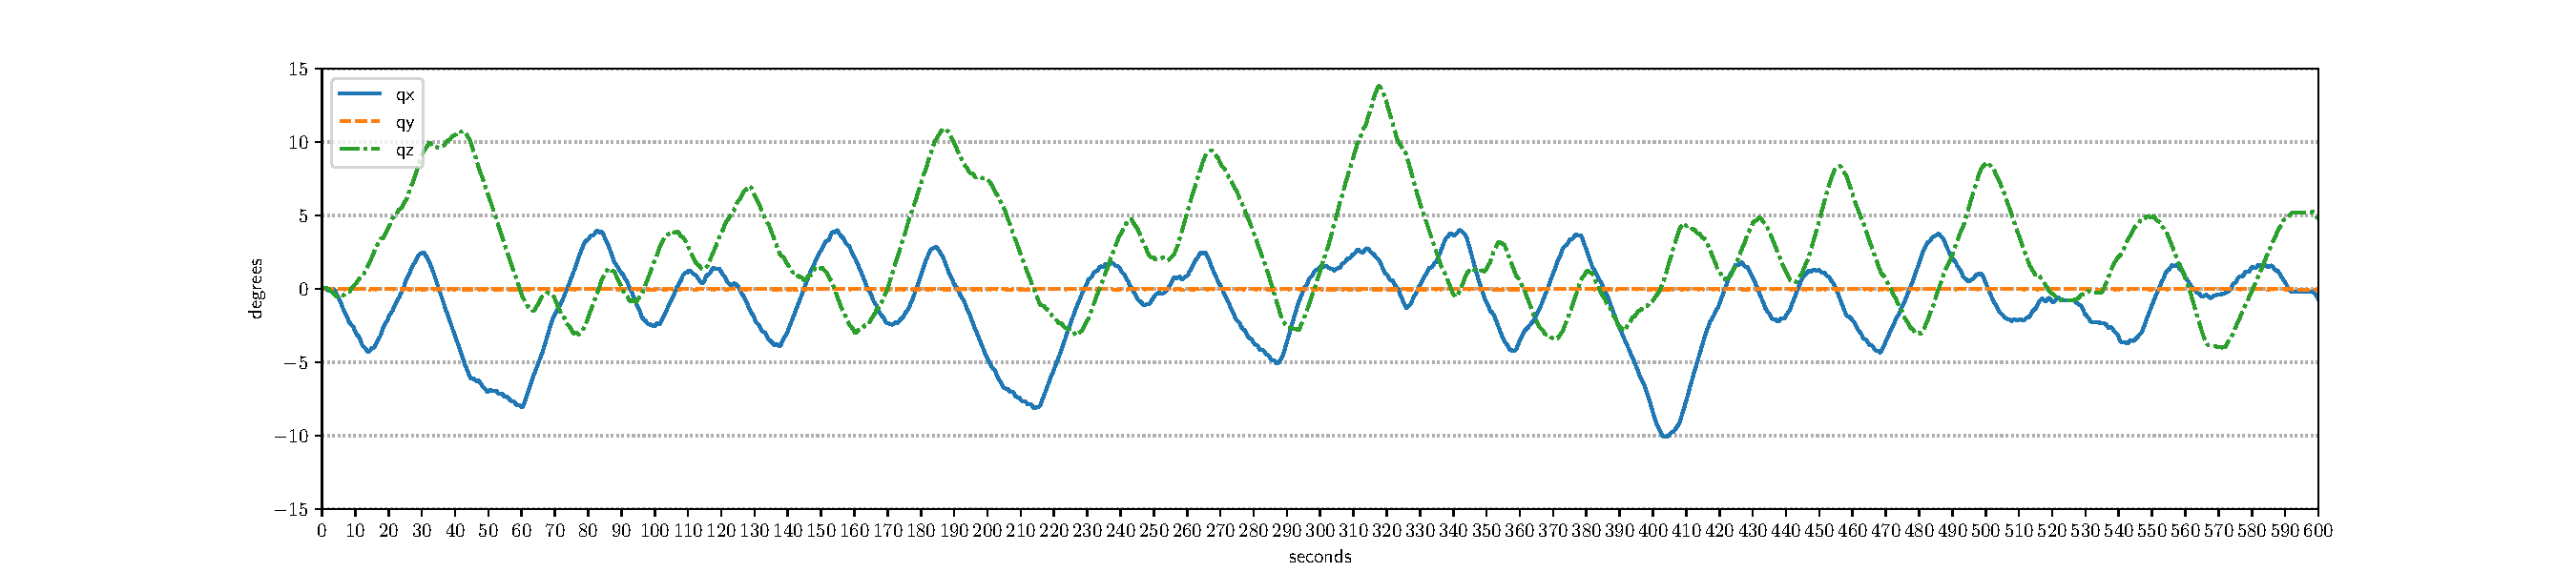
\includegraphics[width=\textwidth]{gfx/Fig-1613-position.pdf}
		\caption{Dataset 1623}
		\label{fig:pos2}
	\end{subfigure}
	\qquad
	\begin{subfigure}[b]{1\textwidth}
		\centering
		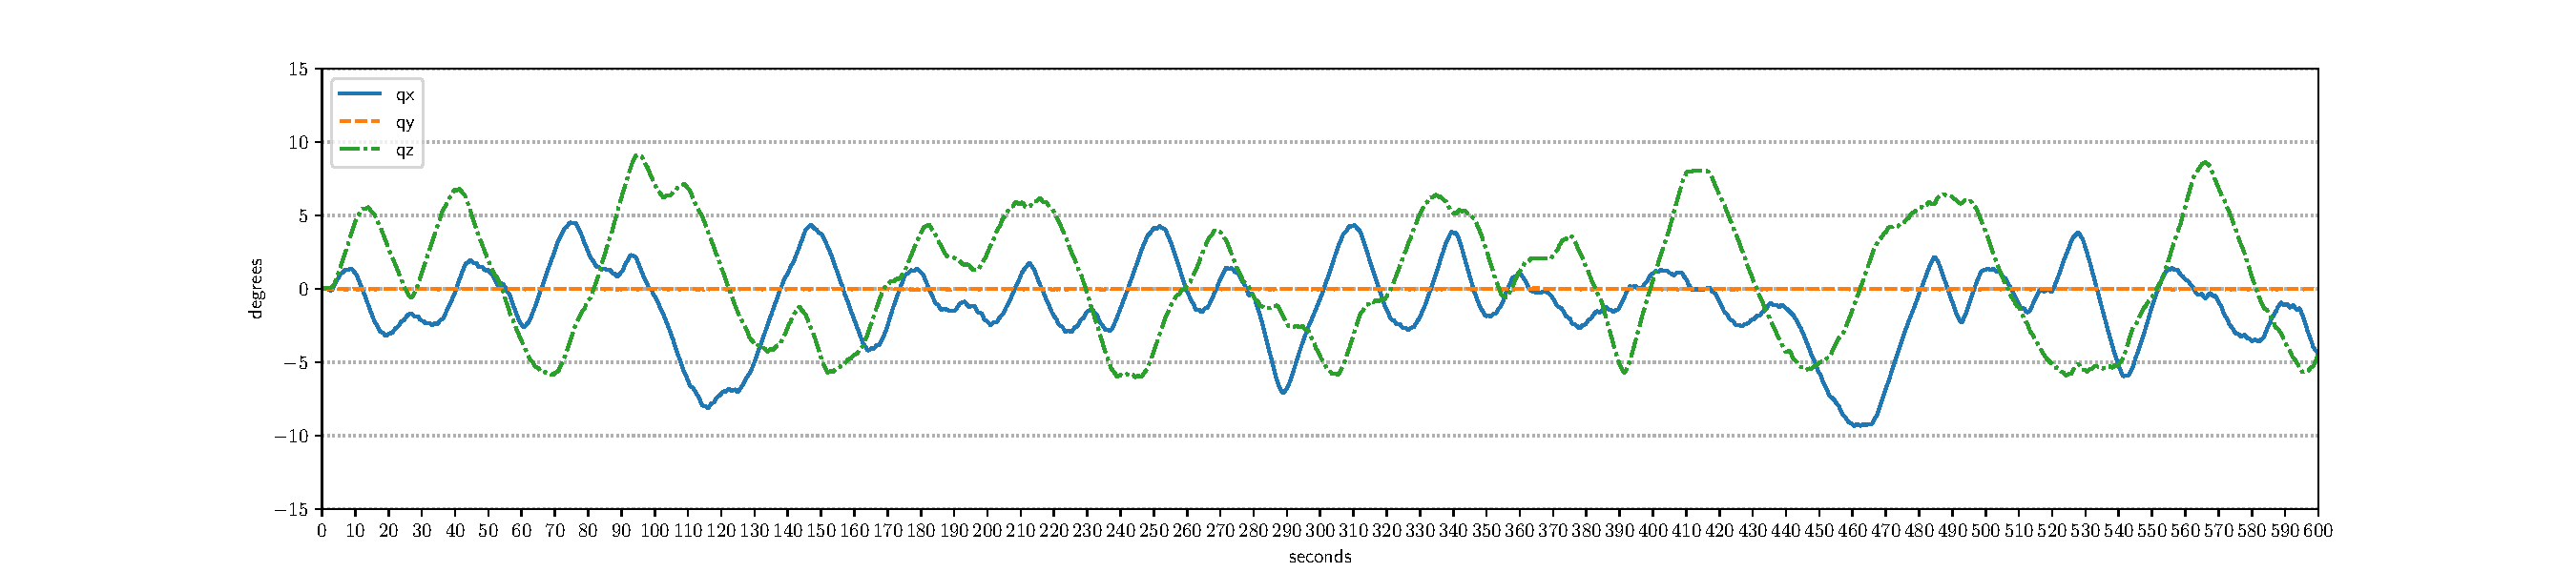
\includegraphics[width=1\textwidth, keepaspectratio]{gfx/Fig-1703-position.pdf}
		\caption{Dataset 1703}
		\label{fig:pos3}
	\end{subfigure}
	\caption{User position plots from obtained datasets (a, b, c).}
	\label{fig:datasets}
\end{figure}
First, let's start with the analysis of user position data. The figures \ref{fig:pos1}, \ref{fig:pos2}, \ref{fig:pos3} show dataset named $1556, 1623$ and $1703$ correspondently. As a matter of fact, plotted dataset were already interpolated on the preprocessing step. Although interpolation was done before data exploration, the details about interpolation can be found in section \ref*{sec:impl:dataset:preprocessing}. The names of datasets means only a $timestamp$ in form $HH:MM$ when a dataset was obtained from HMD in laboratory space. Thus the unique name of $csv$-files on HMD system was guaranteed for the day of experiment. In this thesis the names will be used to identify each of all three datasets. Fig. \ref{fig:datasets} shows only 3 chosen datasets from those obtained in laboratory space. All datasets indicates the same behaviour of VR users with HMD looking on the VV projected in VR space as was found out in works \cite{serhan_kalman, user_behav_volumetric}. The MAE and RMSE metric results are tend to be similar for every dataset during training and testing.

All traces were recorded over 10 minutes long on average 12 minutes. All traces were then shortened to a precise length of 10 minutes to ensure equal data length for the purpose of visualization and analysis. The observations based on the sample traces can be made similar as it done by \textit{Gül et al., 2020} in their work \cite{serhan_kalman}. The user rarely moves along the y-axis. The y-axis shows the vertical movement that the users could make if they sit down or stand up. Based on the data obtained, users walked around a volumetric object in virtual reality and did not make particularly noticeable and prolonged attempts to examine the object at the lower point of the projection on a laboratory's floor since vertical movement requires more effort to crouch down and stand up. The laboratory space where the dataset was obtained was not cluttered with furniture thus users could walk around the volumetric object projected into their HMD. The figure \ref{fig:y_pos} shows an enlarged y-axis in the range from 400ms to 500ms and thus proves there is no significant change in the vertical position of the user.

\begin{figure}[htb]
	\begin{center}
		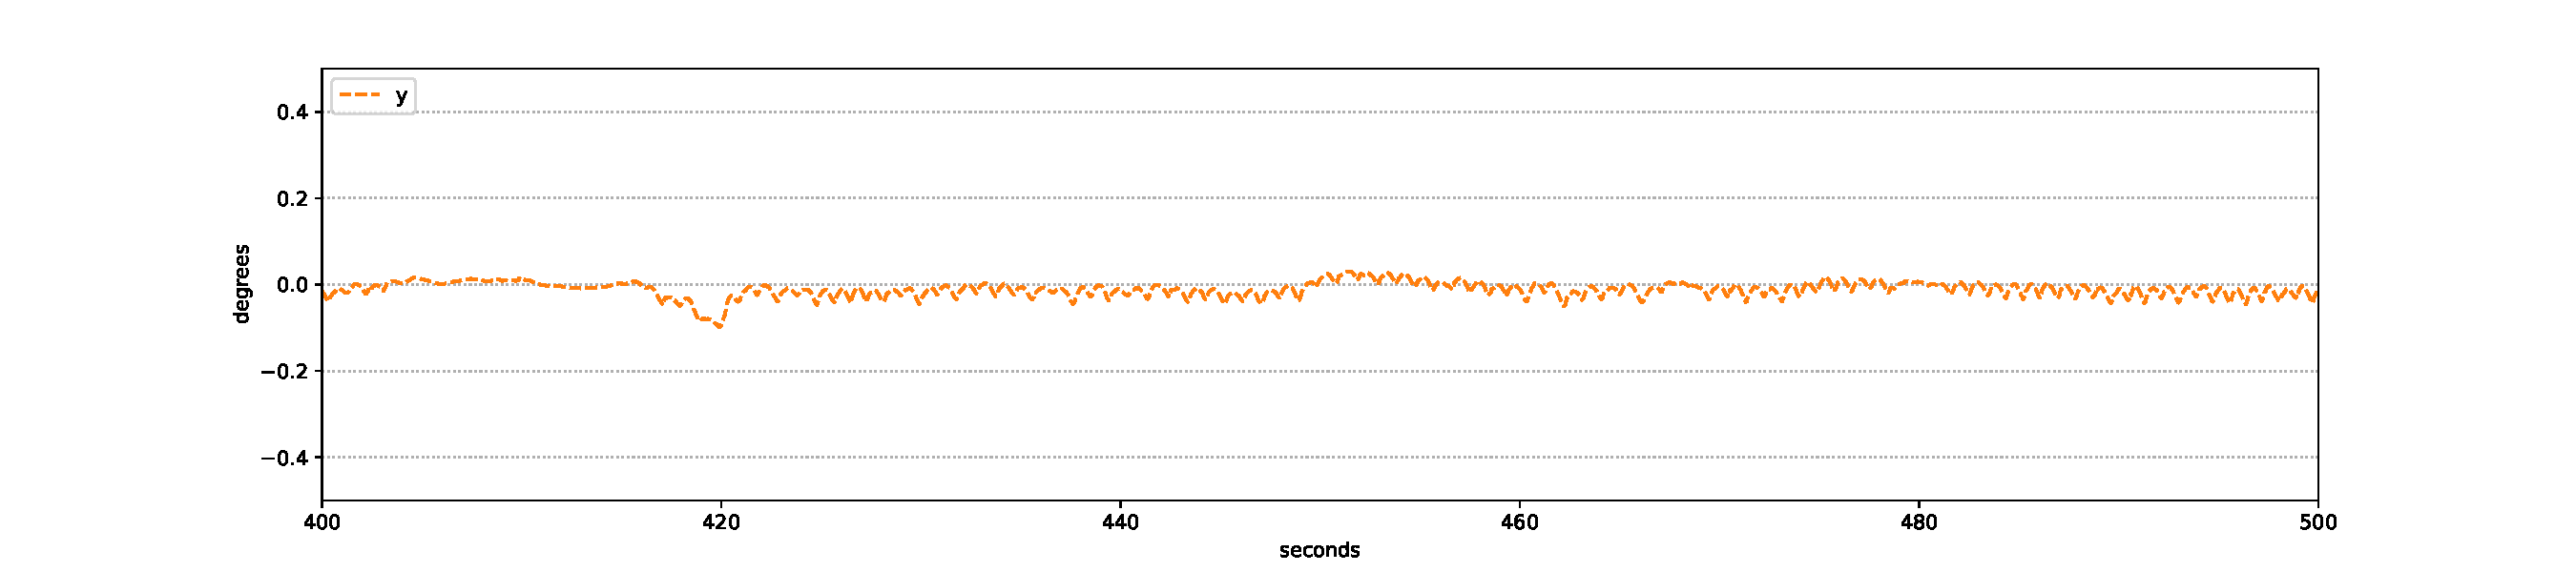
\includegraphics[width=1\textwidth, keepaspectratio]{gfx/Fig-1556-y_position.pdf}
		\caption{\label{fig:y_pos} Changes in the user's position along the Y axis in the range from 400ms to 500ms.}
	\end{center}
\end{figure}

Spatial coordinate systems on Windows (HoloLens runs on the Windows Holographic OS) must be right-handed according to the Microsoft documentation. However Unity documentation points that Unity uses a left-handed convention for its coordinate system and experiments performed in Unity with HoloLens 2 during implementation step proved that spacial coordinates in dataset recorded from left-handed system. In both kinds of coordinate systems, the positive X-axis points to the right and the positive Y-axis points up (aligned to gravity). In recorded dataset positive Z-axis points away from a user. Spatial coordinate systems of HoloLens expresses coordinate values in meters. The mean of position for axes are $X = - 0.71, Y = 0.01, Z = 1.58$ for dataset $1556$. This statistical indicator helps to judge the movement pattern in VR environment projected inside the particular laboratory space. The user's movement along X axis are shifted 0,7 m to the left side in the direction of negative axis. This can be explained by the position of origin of the coordinates when the Unity application was launched. If the application was not launched strictly in the center of the room, but rather closer to the window or wall on one side of the room, then the user had less room space from the side of the window or wall. Y-axis shows no significant change in the movement and thus rather reflects the difference of the HMD position on the head when user made steps walking in the room. Mean of Y-axis of dataset $1556$ shows in average user was about 1,58 m back from the origin of coordinate system. The VV object of a real animated human was placed 3 meters ahead of the user. It seem that users required to step back 1-2 meters to be able to see the whole height of placed VV object respecting the limited Field of view (FoV) of HoloLens 2. Microsoft website\footnote{https://www.microsoft.com/en-us/hololens/hardware} states the headset’s aspect ratio is 3:2, horizontal Field of view (FoV) of 43$^{\circ}$ and a vertical of 29$^{\circ}$. Indeed the standard deviation for axes $X = 3.23, Z = 3.92$ shows that user circled the hologram (VV of a human) with a average distance 3-4 meters looking on the volumetric object from all sides. For Y-axis $Y_{std} = 0.015$ corresponds to a distance deviation from the measured mean when user was walking in the room without significant movement up (like jumping) or down (sitting down on the floor).

%################################################

\subsection{Data preprocessing}
\label{sec:impl:dataset:preprocessing}
As was mentioned in section \ref*{sec:impl:dataset:HL}, the raw sensor data obtained from the HoloLens was unevenly sampled at 60 Hz and had different temporal distances between consecutive samples. The data preprocessing step transforms the data into a format that is more easily and effectively can be processed and visualised. Table \ref{tab:inter_data_pos} shows 20 first rows from the resulting dataset after upsampling the positional data with linear interpolation.
\begin{table}[!ht]
	\footnotesize
	\centering
	\begin{tabular}{|l|l|l|l|}
		\hline
		timestamp & x & y & z \\ [0.5ex] 
		\hline\hline
		0.0 & 0.004954389 & 0.003402365 & 0.01010712 \\ \hline
		5000000.0 & 0.0048331026667 & 0.003308667 & 0.0105062067 \\ \hline
		10000000.0 & 0.00471181633333 & 0.003214633332 & 0.01090523 \\ \hline
		15000000.0 & 0.00459053 & 0.003120769 & 0.01130438 \\ \hline
		20000000.0 & 0.004485576166 & 0.00309903333 & 0.0115486078 \\ \hline
		25000000.0 & 0.00438062233 & 0.00307733667 & 0.011792899 \\ \hline
		30000000.0 & 0.0042756685 & 0.0030556205 & 0.01203707 \\ \hline
		35000000.0 & 0.004170714667 & 0.0030339033 & 0.0122813 \\ \hline
		40000000.0 & 0.00406576084 & 0.00301218867 & 0.01252553 \\ \hline
		45000000.0 & 0.003960807 & 0.002990472 & 0.01276976 \\ \hline
		50000000.0 & 0.00390328375 & 0.00300229975 & 0.0128401975 \\ \hline
		55000000.0 & 0.0038457605 & 0.0030141275 & 0.012910635 \\ \hline
		60000000.0 & 0.00378823725 & 0.00302595525 & 0.0129810725 \\ \hline
		65000000.0 & 0.003730714 & 0.003037783 & 0.01305151 \\ \hline
		70000000.0 & 0.003651043834 & 0.00311298635 & 0.01315696 \\ \hline
		75000000.0 & 0.003571373667 & 0.00318818967 & 0.01326241 \\ \hline
		80000000.0 & 0.003491703003 & 0.003263393 & 0.01336786 \\ \hline
		85000000.0 & 0.003412033332 & 0.0033385963 & 0.01347331 \\ \hline
		90000000.0 & 0.003332363167 & 0.003413799667 & 0.01357876 \\ \hline
		95000000.0 & 0.003252693 & 0.003489003 & 0.01368421 \\ \hline
	\end{tabular}
	\caption{\label{tab:inter_data_pos}Interpolated positional data from HoloLens 2.}
\end{table}

\textit{Gül et al., 2020} obtained the similar raw dataset from same HMD and interpolated it to obtain temporally equidistant samples. Same as it was done in work \cite{serhan_kalman}, the position and velocity data were upsampled using linear interpolation. Spherical linear interpolation was used to interpolate between rotations represented by quaternions and  table \ref{tab:inter_data_rot} lists 20 first rows from the resulting dataset after upsampling the rotational data.

\begin{table}[!ht]
	\footnotesize
	\centering
	\begin{tabular}{|l|l|l|l|}
		\hline
		qx & qy & qz  & qw \\ [0.5ex] 
		\hline\hline
		0.05225104 & -0.0092471 & -0.01470939 & 0.998482825\\ \hline
		0.052829134 & -0.0094018 & -0.01476541 & 0.9984501\\ \hline
		0.053407194	& -0.0095559 & -0.0148214108 & 0.99841708 \\ \hline
		0.053985240 & -0.00971031 & -0.0148774088 & 0.9983836 \\ \hline
		0.054563231 & -0.0098646 & -0.0149333515 & 0.99834990 \\ \hline
		0.054967034 & -0.0099280 & -0.0147404755 & 0.99832999 \\ \hline
		0.055370826 & -0.0099914 & -0.014547596 & 0.998309876 \\ \hline
		0.055774607 & -0.0100548 & -0.0143547143 & 0.998289554 \\ \hline
		0.056178376 & -0.0101182 & -0.0141618293 & 0.9982690 \\ \hline
		0.0565821344 & 0.0101816 & -0.01396894 & 0.998248298 \\ \hline
		0.0568467445 & -0.0102414 & -0.01378002 & 0.99823527 \\ \hline
		0.0567612581 & -0.01029217 & -0.01360108 & 0.998242075 \\ \hline
		0.0566757694 & -0.01034289 & -0.013422148 & 0.998248830 \\ \hline
		0.0565902782 & -0.01039361 & -0.013243212 & 0.9982555436 \\ \hline
		0.0565037268 & -0.01044992 & -0.0130706110 & 0.998262133 \\ \hline
		0.0563820024 & -0.010691806 & -0.01310865 & 0.998265955 \\ \hline
		0.0562602738 & -0.010933688 & -0.01314669 & 0.998269703 \\ \hline
		0.0561385409 & -0.011175569 & -0.013184732 & 0.9982733762 \\ \hline
		0.0560168039 & -0.011417450 & -0.013222770 & 0.99827697 \\ \hline
	\end{tabular}
	\caption{\label{tab:inter_data_rot}Interpolated rotational data from HoloLens 2.}
\end{table}

\begin{figure}[htb]
	\begin{center}
		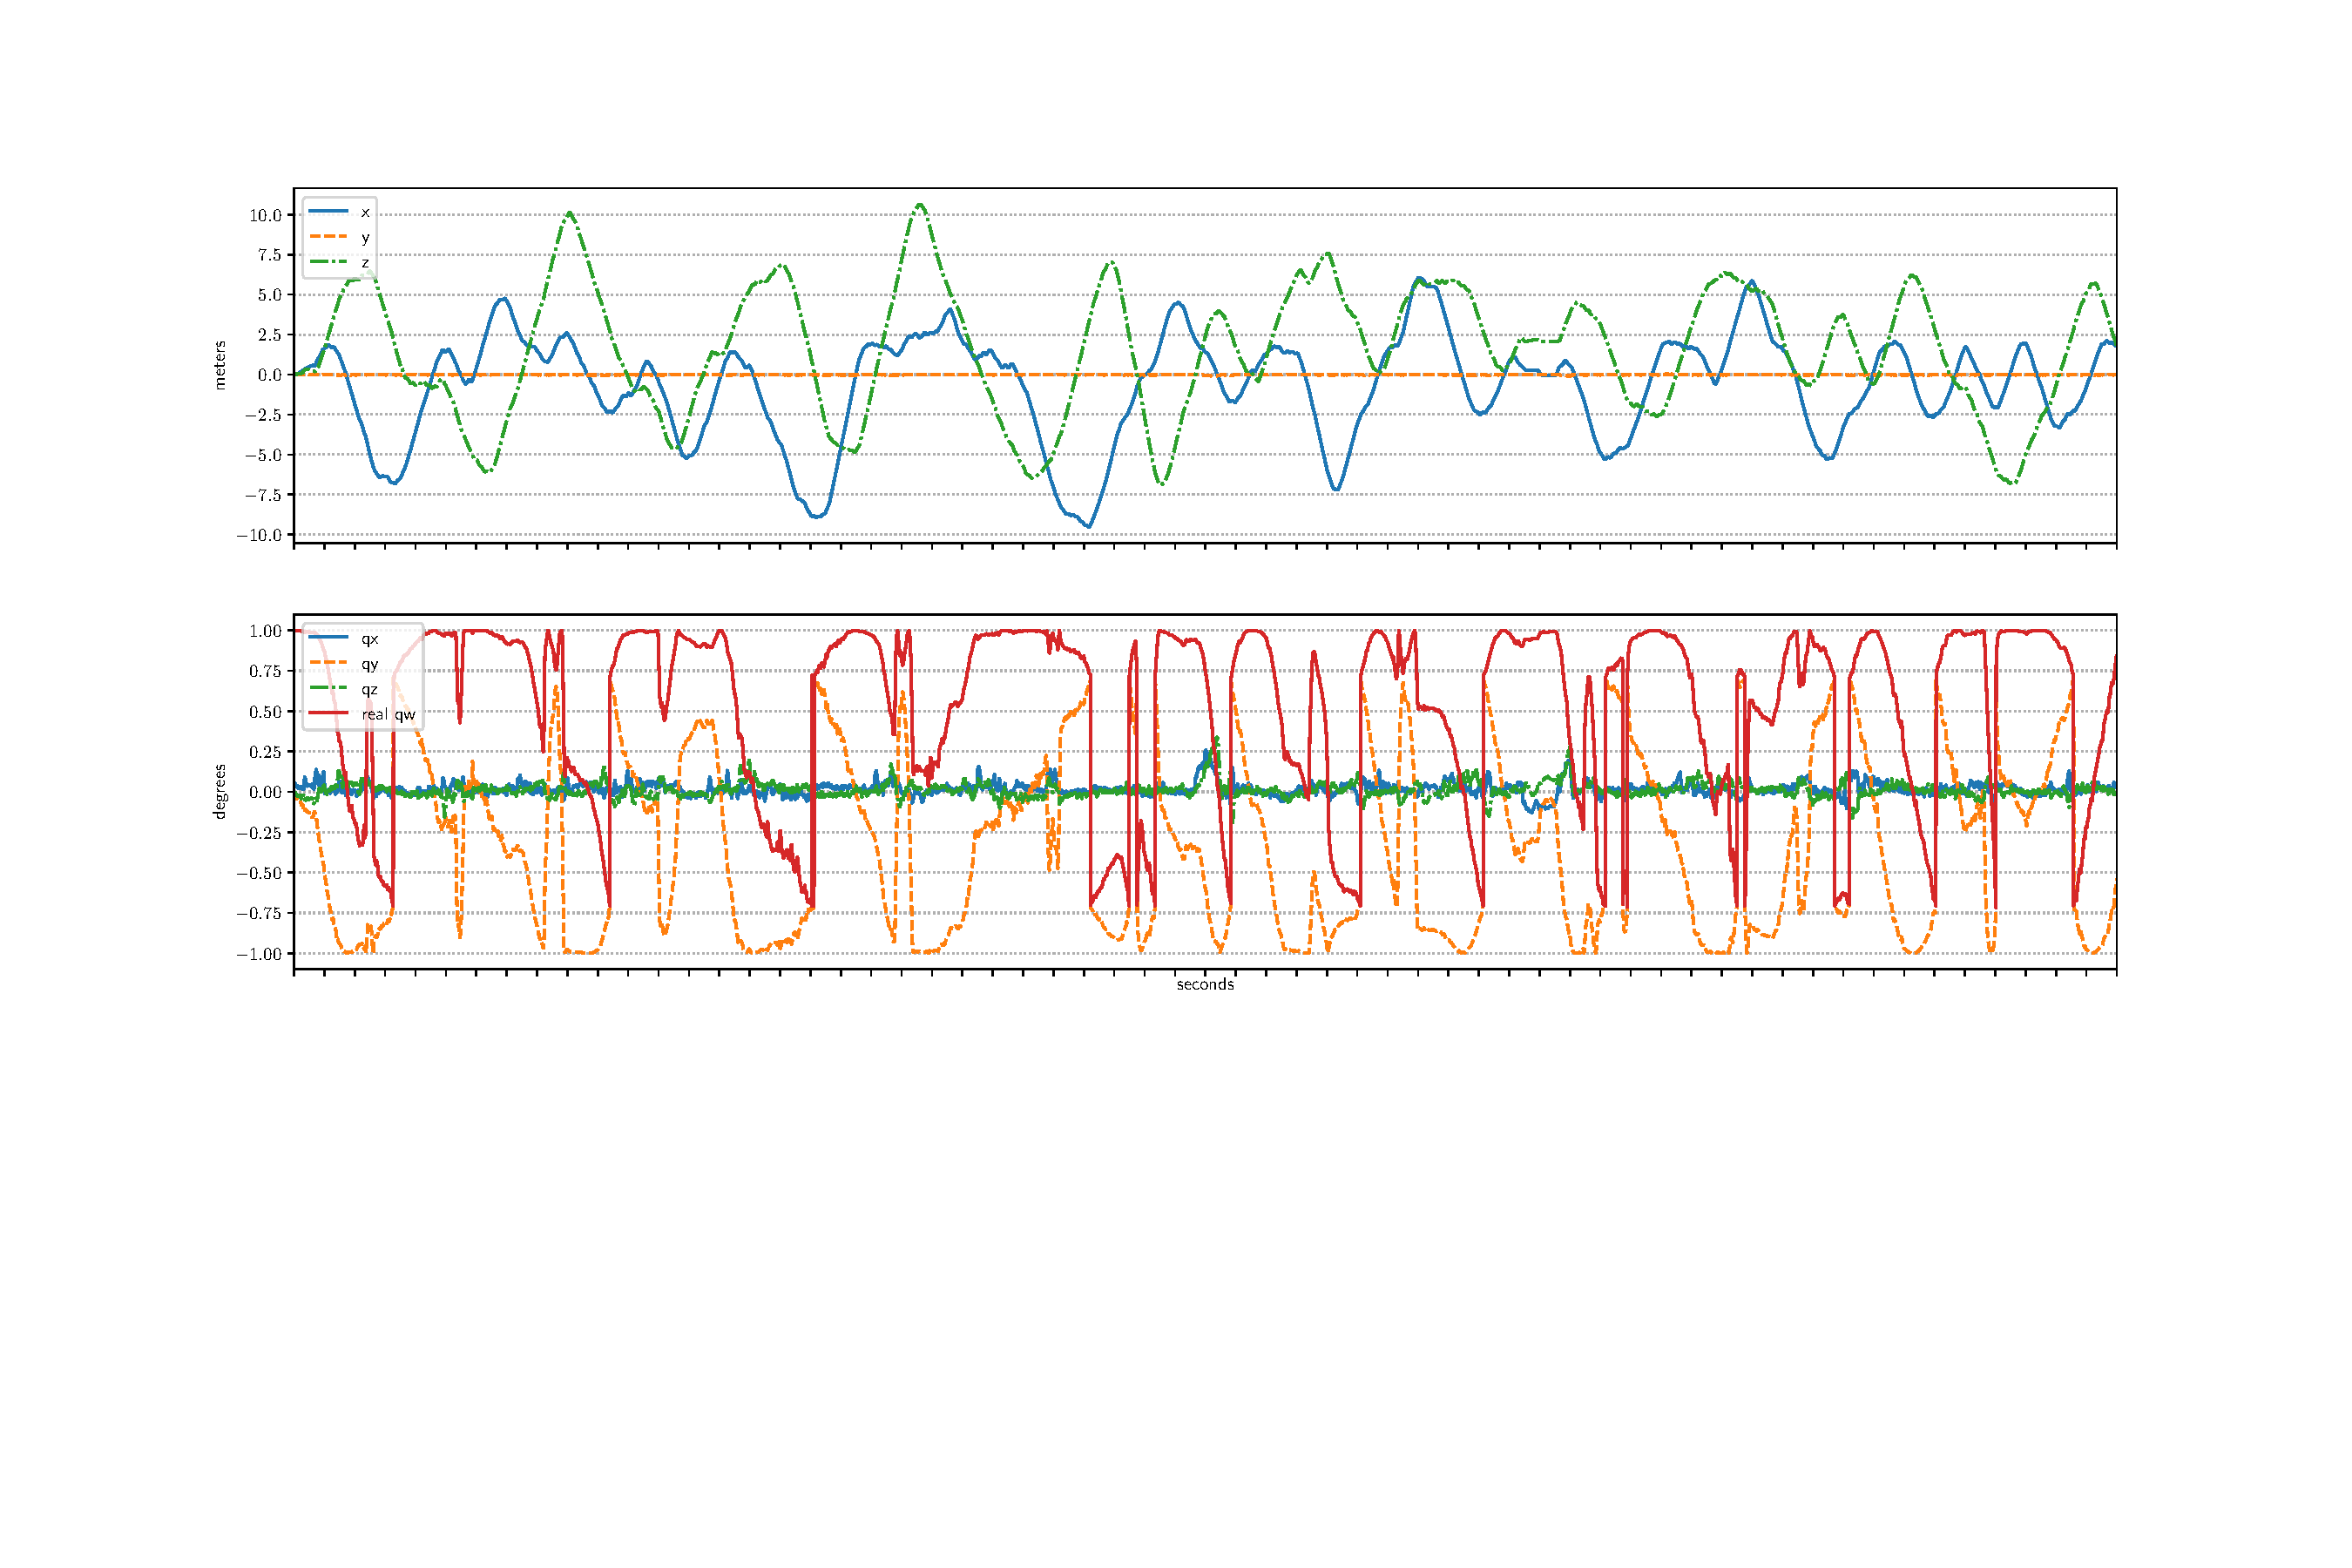
\includegraphics[width=1\textwidth, keepaspectratio]{gfx/Fig-1556-interpolated_2.pdf}
		\caption{\label{fig:inter_data}Interpolated 6-DoF dataset's user position and orientation in quaternions.}
	\end{center}
\end{figure}

After the interpolated dataset was plotted as figure \ref{fig:inter_data}, the important observations based on the sample trace could be done. While the user position data plots look appropriate for machine learning algorithms, the graph with orientation shows data that is not the perfect case for usage with machine learning technologies and could decrease the prediction rate. The real part $qw$ and the component $qy$ of quaternion have obviously discontinuous (sharp change of sign) making it hard for a predictor to learn. A orientation on quaternions is used in training, thus this data requires a few additionally preprocessing steps. Usually, when doing calculation with quaternions, quaternions must be normalized to a unit length in order to represent valid rotations \cite{principles_robot_motion_book}. The normalized quaternion can be calculated using formula:
\begin{equation}
U_g = \frac{q}{|| q ||} = \frac{w}{|| q ||} + i \cdot \frac{x}{|| q ||} + j \cdot \frac{y}{|| q ||} + k \cdot \frac{z}{|| q ||}
\end{equation}

where $|| q || $ is a magnitude and can be found with formula:
\begin{equation}
|| q || = \sqrt{w^2 + x^2 + y^2 + z^2 }
\end{equation}

During experiments with quaternions in dataset obtained from HoloLens 2, was detected that quaternion magnitudes $|| q ||$ in HoloLens dataset are equal to 1. Thus data came from HMD already normalized, so that a quaternion in dataset kept the orientation as it was during user's movement with a magnitude equal to 1.0.

Next, quaternions between neighboring points in obtained dataset represent the very similar orientation made by user wearing HMD step by step. The orientation plot on figure \ref{fig:norm_data} has discontinuities that can be seen on $qw$ line. As a consequence of the discontinuity (sharp change of line from negative to positive area with the same amplitude) the two neighboring quaternions with similar rotation have significant 4D vector space between them. It makes prediction worse what can be proved by RMSE and MAE rotation metrics. Flipping the sign will not affect the rotation, but it will ensure that there are no large jumps in 4D vector space when the rotation difference in rotation space (SO(3)) is small. If negative component of quaternions will be flipped into positive then the dataset, representing same rotation without creating an artificial discontinuity in the space, will be available for model training. 

\begin{figure}[htb]
	\begin{center}
		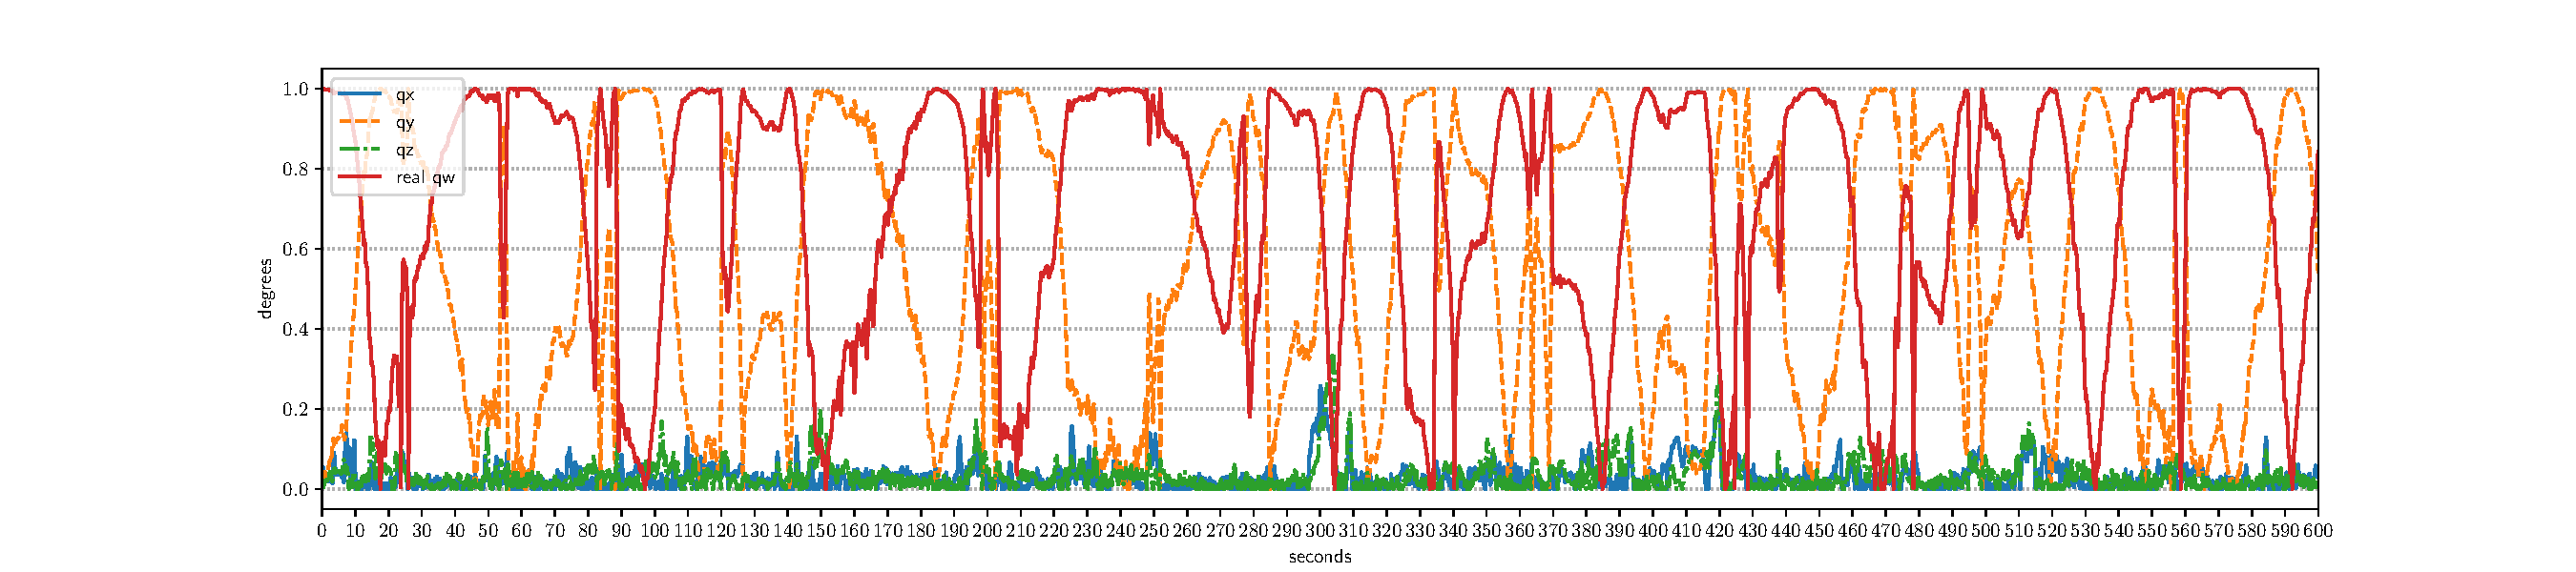
\includegraphics[width=1\textwidth, keepaspectratio]{gfx/Fig-1556-quaternions_flipped.pdf}
		\caption{\label{fig:norm_data} Quaternions from 6-DoF dataset's flipped if their real part is negative.}
	\end{center}
\end{figure}

 The figure \ref{fig:compare} represents quaternions of the original interpolated dataset on the upper part of the plot and the normalized flipped quaternions on the lower part of the plot. The quaternion's components were flipped only if the if their real part became negative. Different to figure \ref{fig:norm_data} the limit of y-axis is set to [-1, 1] on figure \ref{fig:compare} so that the result of inverting of quaternion is easy co compare to original data. Figure \ref{fig:norm_data} shows plotted data with length of 20 seconds in range 162 - 182 s from both datasets.
\begin{figure}[htb]
	\begin{center}
		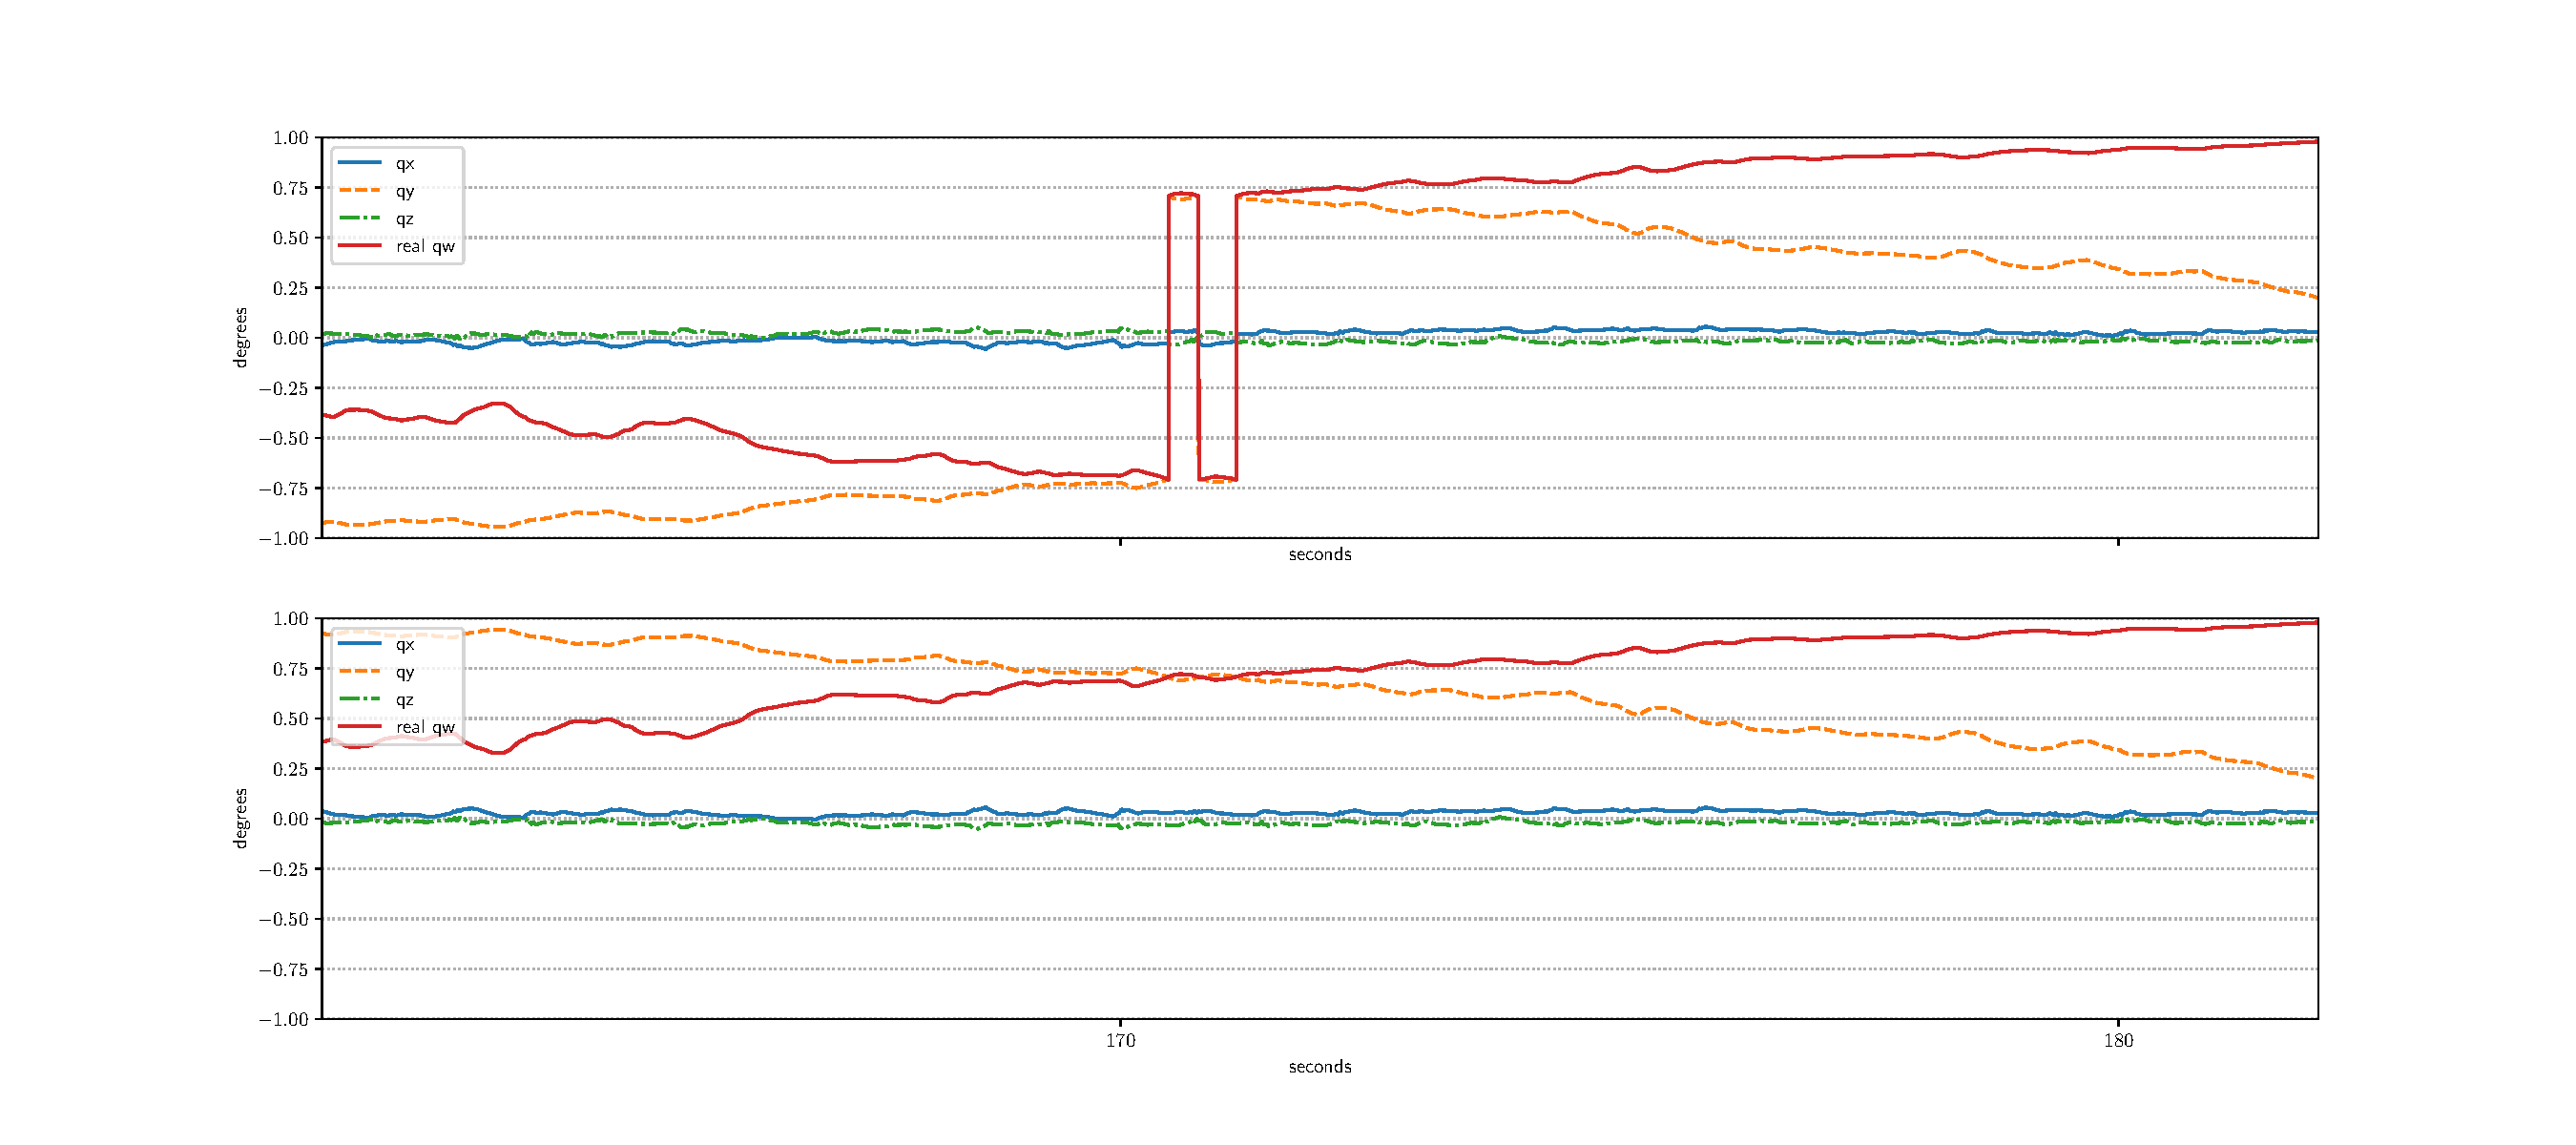
\includegraphics[width=1\textwidth, keepaspectratio]{gfx/Fig-1556-compare.pdf}
		\caption{\label{fig:compare} Enlarged quaternion plot with breaks omitted.}
	\end{center}
\end{figure}

Thus the two representations of quaternions were blended into one data set, omitting to discontinuities in the time series as can be seen presented on Figure \ref{fig:norm_data}. Indeed, the RMSE and MAE rotation metrics were improved when model was trained with dataset with quaternions without sharp sign changes. More information can be found in section \ref{sec:eval:experiments}.
%''########################################

\newpage
\section{Model}
\label{sec:impl:model}
The section describes the inputs and architecture of evaluated LSTM, GRU and Bidirectional GRU models. A model itself is a mathematical representation that produces expected output based on a given input. 
\subsection{Inputs and outputs}
\label{sec:impl:model:inputs}
The correct chosen model can discover and learn the patterns in the input dataset while being trained in order to predict a new data after training. In the sections \ref{sec:impl:dataset:explor} and \ref{sec:impl:dataset:preprocessing} the obtaining and structure of 6-DoF is covered. After data preprocessing step, the interpolated dataset with flipped negative quaternion was used for model training. The dataset itself can not be used with model directly and a sequence data must be prepared to feed as an input into an RNN model. The 6-DoF dataset is a two-dimensional array. The first dimension of 6-DoF dataset represents the number of timesteps of the recorded dataset. The second dimension represents the number of features of input sequence. During data collection a 6-DoF dataset with 10 features was created. Recorded in dataset features are position $(x, y, z)$, orientation $(qx, qy, qz, qw)$ and velocity $(x, y, z)$ data. 

However PyTorch’s LSTM and GRU models expect all of their inputs to be 3D tensors. Thus 2D data must be converted into 3D data. The meaning of the axes of these tensors is important. The first axis by default is the sequence itself, the second indexes instances in the batches, and the third indexes features of the input. By specifying PyTorch's parameter $batch first = true$ the input and output tensors were provided as $(batch, seq, feature)$ instead of $(seq, batch, feature)$. This change does not apply to hidden or cell states and thus tensor containing the initial hidden for each element in the batch must be initialized as $(D * layers, batch, hidden)$. $D$ is 1 for LSTM and GRU Models and equal to 2 for their bidirectional variant. 

Usually in machine learning dataset will be split randomly, as there’s no dependence from one observation to the other. With time series representing user position and rotation the is not a case and data have to split with respect to time dependencies. The 6-DoF contains a positional data without any seasonal characteristic and there is no obvious way to split data in groups. It is decided to split dataset into three datasets: training, validation and test dataset. The split ratio is 60:20:20 for each corresponding dataset. Thus first 60\% of data used for training, next 20\% for validation and the rest 20\% for testing. No dimensional shuffle was applied to keep the original time dependencies. During training loop on each epoch model trained on training dataset in $train()$ mode that allows the learning process with updating of model weights. In the end of each epoch model was explicitly set into evaluation mode by calling the $eval()$ function mode to turn off gradients computation and validated on the validation dataset. When model repeatedly trained for 500 epochs, model predicted a new data on never seen before test dataset. 

The last step to prepare 6-DoF dataset to be used as model input is using time steps as features. Having a historical data of user position and orientation, the next value, $X(t+n)$ must be predicted by a model from the previous n observations $Xt, X+1$, ..., and $X(t+n-1)$. Since the future values that must be predicted already recorded in the dataset, a sliding-window approach can use prior time steps to predict the next time step and thus turn a time series dataset into a supervised learning problem. With a simple for-loop lagged observations can be created from input by shifting the values in a column by n times and removing the first n columns. The original dataset was interpolated using linear interpolation for position data and SLERP is used for quaternions. Thus, interpolated dataset is an evenly-sampled dataset with a sampling rate of 200 Hz (5 ms). The LAT of 100 ms is used for evaluation. Thus 20 future values correspond the $LAT = 100 ms$ must be predicted by LSTM and compared with real data to evaluate the prediction. 

Finally, the spit datasets with added sliding window were exported in standard binary $npy$-files format of NumPy. The format stores all of the shape and dtype information necessary to reconstruct the array correctly even on another machine with a different architecture. Thus the spitting of dataset is not required every time when model trains with different hyperparametes on GPU cluster.
 
\subsection{LSTM Model}
\label{sec:impl:model:arch:lstm}
Recurrent neural networks have recently shown promising results in many machine learning tasks, especially when input and/or output are of variable length and are coming as time series with a sequential order. Unfortunately, the known problem of RNN that was observed many years ago by e.g., \textit{Bengio et al., 1994} that it is difficult to train RNNs to capture long-term dependencies because the gradients tend to either vanish (most of the time) or explode (rarely, but with severe effects) \cite{rnn_difficults}. New approaches are needed to be implemented to reduce the negative impacts of this issue. Since traditional recurrent unit overwrites its content at each time-step, a LSTM unit is able to decide whether to keep the existing memory via the introduced gates. The Long Short-Term Memory (LSTM) has a number of minor modifications \cite{empirical_evaluation} since it was initially proposed in work \cite{lstm_orig}.
Analysis done by \textit{Qian et al., 2016} indicates that in the short term users’ head movement can be predicted with accuracy > 90\% by even using simple methods such as linear regression \cite{cellular_opt}. However in the longer term it is more difficult to achieve the good result and the average accuracy drops to about 70\% \cite{cellular_opt}. Thus LSTM model was chosen to evaluate with the 6-DoF dataset based on long term dependencies of the data. 

Since LSTM is a special kind of RNN, the RNN architecture will be briefly introduced first. RNN block consist of single computation layer with $tanh$ activation function that is used to help regulate the values flowing through the network. The tanh function squishes values to always be between -1 and 1. RNN has $h_{t}$ function of the previous cell state $h_{t-1}$ and current input$ X_{t}$. The architecture of LSTM is complexer and consists of several computational blocks that control information flow of information through the cell. The key building block behind LSTM is a structure known as $gates$. They allow LSTM to avoid the weight conflict when making decision which information from the past and current timestamp is important for correct mapping inputs to outputs. In other words, network can decide how to use gates when it is needed to keep or override the information in memory cell or access the current memory cell \cite{lstm_orig}. 

\begin{figure}[htb]
	\begin{center}
		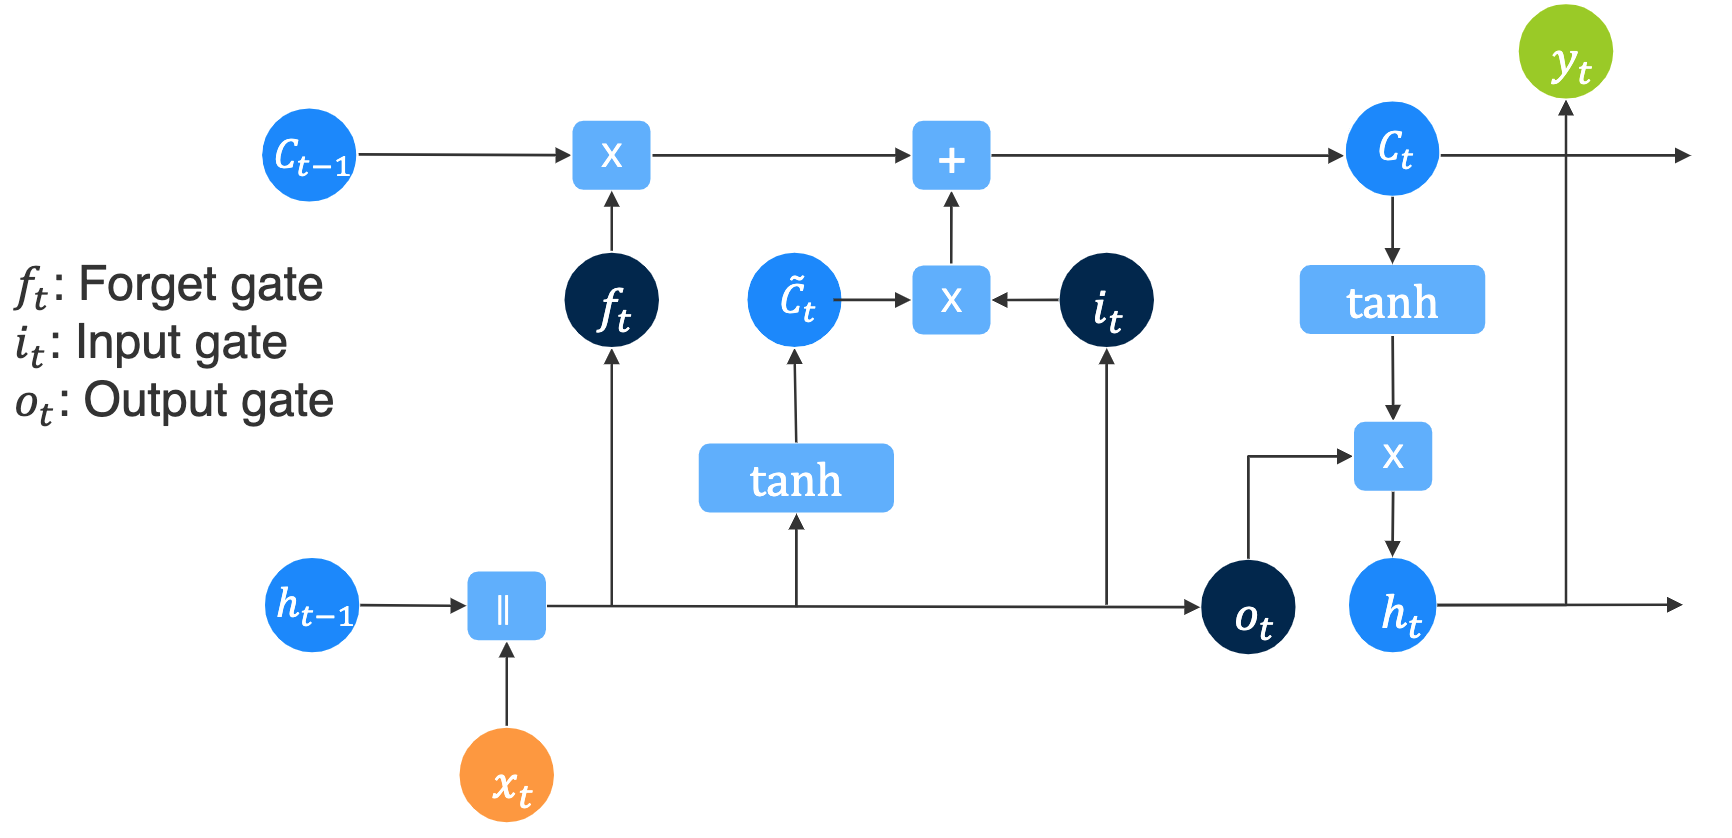
\includegraphics[width=1\textwidth, keepaspectratio]{gfx/lstm.png}
		\caption{\label{fig:lstm}Long Short-Term Memory.}
	\end{center}
\end{figure}
The LSTM architecture is illustrated\footnote{Source: Prof. Dr. Tim Landgraf, Lecture 13: Recurrent Neural Networks, WS 20/21: Machine Learning} on Fig. \ref{fig:lstm}. Using first gate $f_t$ model decides which information should be omitted from the cell in that particular time step. The sigmoid function uses the previous state (ht-1) along with the current input xt and computes the cell state using formula:
\begin{equation}
f_t = \sigma (W_{if}x_t + b_{if} + W_{hf}h_{t-1} + b_{hf})
\end{equation}
where $f_t$ is the forger gate, $h_{t}$  is the hidden state at time t, $h_{t-1}$ is the hidden state of the layer at time $t-1$ or the initial hidden state at time $0$, $\sigma$ is the sigmoid function. All LSTM gates have $sigmoid$ activations that  is similar to the $tanh$ activation but squishes values between 0 and 1. This function is useful for forgetting the information since any number getting multiplied by 0 is 0 and thus disappears from cell state. 

With $i_t$ cell state $c_t$ will be updated. First, the previous hidden state and current input are passed into a sigmoid function on input gate:
\begin{equation}
i_t = \sigma (W_{ii}x_t + b_{ii} + W_{hi}h_{t-1} + b_{hi})
\end{equation}
The transformed values between 0 and 1 meaning 0 means not important, and 1 means important will be multiplied on cell gate $\tilde{c}_t$ with the tanh output of the hidden state and current input:
\begin{equation}
\tilde{c}_t = tahn (W_{ig}x_t + b_{ig} + W_{hg}h_{t-1} + b_{hg})
\end{equation}
New cell state first gets pointwise multiplied by the forget vector anf if these values near 0 they will be dropped from the cell state. The result from the input gate is pointwise added und thus new cell state is created with values that the neural network finds relevant.
\begin{equation}
c_t = f_t \odot c_{t-1} + i_t \odot \tilde{c}_t
\end{equation}
The output gate is the last in LSTM calculations and decides what the next hidden state should be. Hidden state is also used to make a prediction because it contains information of previous inputs and thus helps to learn long term dependencies. The sigmoid function gets previous hidden state and the current input and tanh function gets the newly calculated cell state. And similar to previous step tanh output with the sigmoid output are multiplied to decide what information the hidden state should carry. The new cell state and the new hidden is then carried over to the next time step.
\begin{equation}
o_t = \sigma (W_{io}x_t + b_{io} + W_{ho}h_{t-1} + b_{ho})
\end{equation}
\begin{equation}
h_t = o_t \odot tahn(c_t)
\end{equation}

Model implementation, training loop and evaluation are done in Python using PyTorch. Model has input $[batch, sequence, features]$ with sequence equal to 20 last values what corresponds to 100 ms of historical data and 10 features that contain 3 positional, 4 rotation and 3 velocity columns. The batch size was set to $2^{7}$. The hidden dimension set experimentally after parameters grid search on GPU Cluster to be equal 512. Adam optimization algorithm is used, the maximum number of epochs was set to 500, early stopping technique (patience = 7, min. delta = 0,05) was used to avoid overfitting. Additionally, the learning rate was decreased by 50\% from initial value of 0.0001 every 30 epochs. The learning rate is a parameter that determines how much an updating step influences the current value of the weights. Adjustable learning rate was proposed in works \cite{delay_compensation_360, telepresence} and implementing this option had improved prediction and allowed model to learn patterns correctly without overfitting. Weight decay of Adam optimiser experimentally is set to a small value of $1e-12$ . Thus this additional term in the weight update rule less causes the weights to exponentially decay to zero, large weights were less penalizes and model could successfully learn the long term dependencies and thus constantly decrease both training loss and validation loss  and stabilize them at a specific point. 

The high performance was achieved event without additional activation functions with simple one-layered architecture represented below:
\begin{lstlisting}[caption={One-layered LSTM with sliding window},captionpos=b]
LSTMModel1(
(lstm): LSTM(10, 512, batch_first=True)
(fc): Linear(in_features=512, out_features=7, bias=True)
==================================================================
Layer (type:depth-idx)          Output Shape         Param #
==================================================================
LSTMModel1                       [128, 20, 7]              --
	--- LSTM: 1-1            [128, 20, 512]     1,073,152
	--- Linear: 1-2          [128, 20, 7]           3,591
==================================================================
Total params: 1,076,743
Trainable params: 1,076,743
Non-trainable params: 0
==================================================================
\end{lstlisting}

Since only position and rotation data of similar range is used in 6-DoF dataset, no scaler for the features is applied.  Experiments showed that normalization of values between [0..1] and between [-1..1] results to higher MSE and RMSE. Already preprocessed interpolated datasets with flipped negative quaternions is loaded in with respect to sequential order as training, validation and test dataset from $npy$-files. Additional extended LSTM architectures were implemented and tried with HoloLens 2 6-DoF dataset. For example, the non-linear activation functions $ReLU$ and $Mish$ were tried in order to get more sensitivity to the activation sum input and avoid easy saturation. Thus the nodes in model should be only deactivated if the output of is less than 0. Model variant with $ReLU$ experimentally resulted to produce higher MAE and RMSE compared to LSTM1 and therefore was rejected for a final deployment. Since LSTM2 Model has the similar architecture as following afterwards LSTM3, it is not listed separately 

LSTM3 uses a new activation function $Mish$ that was presented in machine learning scene in 2019 in work \cite{mish} and is a self-regularized non-monotonic activation function which can be mathematically defined as $f(x)=xtanh(softplus(x))$. Mish is a smooth, continuous activation function and allows to have better gradient flow compared to ReLU that tends to have a lot of sharp transitions \cite{mish}. The LSTM3 model improved MAE and RMSE mertics. Model's batch size changed to $2^{10}$. Additional linear layer with additional $Mish$-function is added in order to double the hidden size of LSTM. Weight decay of Adam optimiser is experimentally set to $3e-14$ with LSTM3 model.
 
\begin{lstlisting}[caption={LSTM3 with Mish activation function},captionpos=b]
LSTMModel3(
(lstm): LSTM(10, 512, batch_first=True)
(mish_1): Mish()
(fc_1): Linear(in_features=512, out_features=1024, bias=True)
(mish_2): Mish()
(fc_2): Linear(in_features=1024, out_features=7, bias=True)

==================================================================
Layer (type:depth-idx)                   Output Shape              Param #
==================================================================
LSTMModel2                   [1024, 20, 7]              --
	--- LSTM: 1-1        [1024, 20, 512]            1,073,152
	--- Mish: 1-2        [1024, 20, 512]            --
	--- Linear: 1-3      [1024, 20, 1024]           525,312
	--- Mish: 1-4        [1024, 20, 1024]           --
	--- Linear: 1-5      [1024, 20, 7]              7,175
==================================================================
Total params: 1,605,639
Trainable params: 1,605,639
Non-trainable params: 0
==================================================================
\end{lstlisting}

LSTM4 Model is a three-layered stacked LSTM with introduced additional dropout  added after all but last recurrent layer and Mish activation function. This design decision is made in order to try whether adding more components to the neural network could mean the improvement upon simpler model on 6-DoF dataset. By adding more LSTM layers the model parameters that have to be trained were increased in 5 times from 1,605,639 to 7,901,191 trainable parameters. When the model parameters are getting large in count, the model gets more complex, having hard time fitting on the training instances as it needs to optimize parameters in a way that can optimally fit the training instances. The time need for training increased noticeable even on GPU Cluster. Finally, LSTM4 resulted in significant higher MAE and RMSE metrics and thus this architecture is rejected.  

This models LSTM1 and LSTM3 are considered to be the best evaluated LSTM models that can predict the future data based on past 20 values (100 ms) in 6-DoF VR environment using sensor data from HMD for LAT of 100 ms. Although sufficient results for prediction and low MAE and RMSE metrics are already obtained with LSTM model, the GRU and bidirectional models will be implemented in order to evaluate their performance and potentially to find the better model architecture. 

\subsection{GRU Model}
\label{sec:impl:model:arch:gru}
Another approach called a gated recurrent unit (GRU) can adaptively capture dependencies of different time scales without having a separate memory cells \cite{empirical_evaluation}. It is similar to an LSTM, but only has two gates - a reset gate and an update gate. Although architecture does not provide an output gate, with fewer parameters it can generally easier and faster be trained than LSTM.  GRU Model can catch the long-term dependencies in the data obtained from HMD that are otherwise are hidden by the effect of short-term dependencies from the standard RNN models. This chapter decribes GRU model that implemented to predict future values with 6-DoF dataset obtained from HoloLens 2. \\

\begin{figure}[htb]
	\begin{center}
		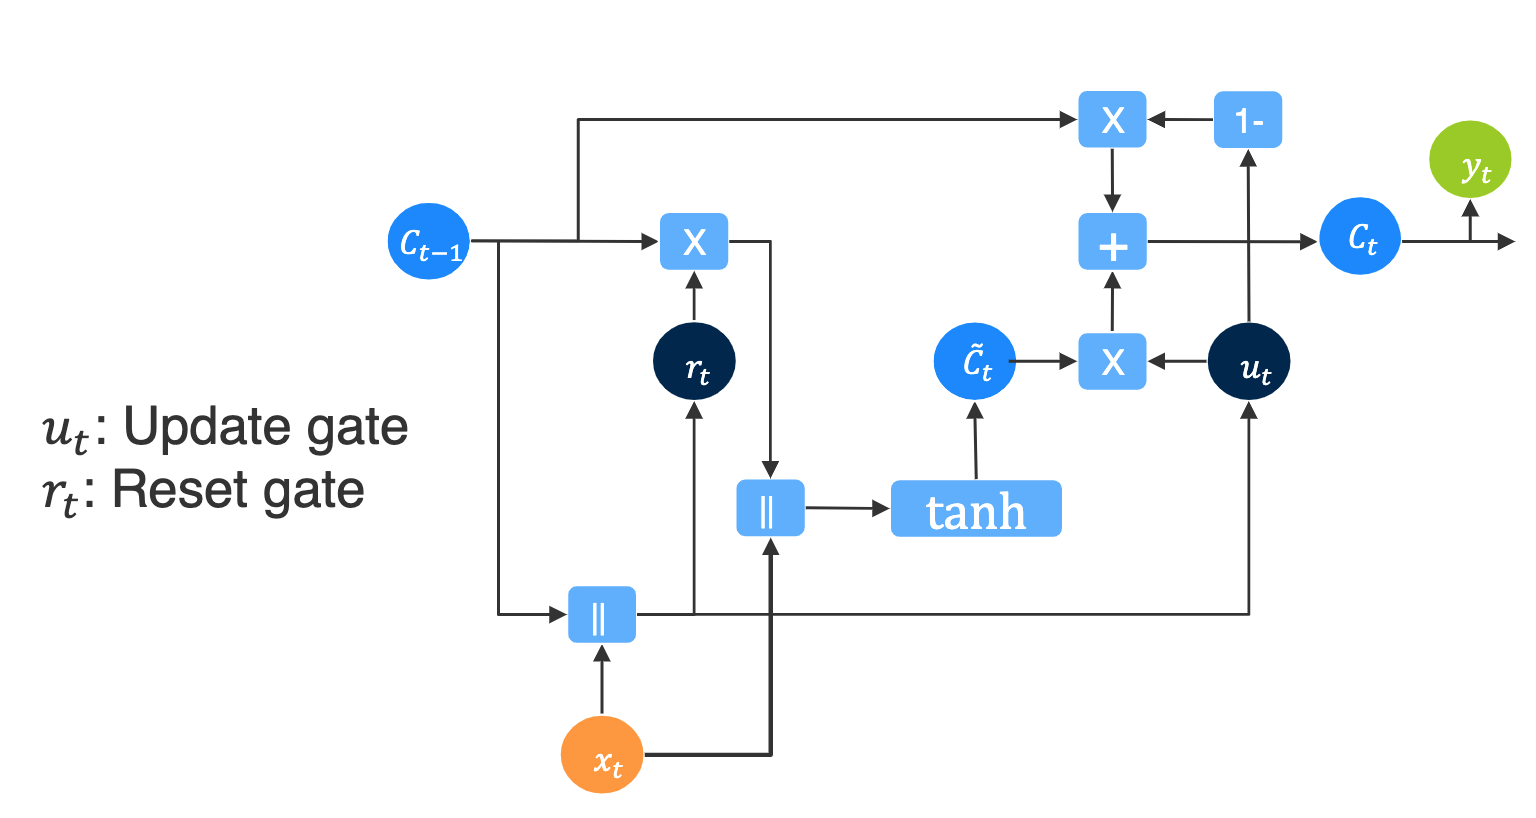
\includegraphics[width=1\textwidth, keepaspectratio]{gfx/gru.png}
		\caption{\label{fig:gru}Gated Recurrent Unit.}
	\end{center}
\end{figure}

The GRU architecture is illustrated\footnote{Source: Prof. Dr. Tim Landgraf, Lecture 13: Recurrent Neural Networks, WS 20/21: Machine Learning} on Fig. \ref{fig:gru}. GRU avoids the vanishing gradient problem of a standard RNN with only two gates that decide what information should be passed to the final output. The update gate plugs $x_t$ into the network unit and multiplied with its own weight $W_{iz}$. The same multiplication is done with previous hidden state $h_(t-1)$ that has its own weight $W_{hz}$. Both results are added together and a sigmoid activation function is applied to squash the result between 0 and 1. The mathematical expression of this calculation is as following:
\begin{equation}
z_t = \sigma (W_{iz}x_t + b_{iz} + W_{hz}h_{t-1} + b_{hz})
\end{equation}
where  $z_t$ is an update gate, $h_{t}$  is the hidden state at time t, $h_{t-1}$ is the hidden state of the layer at time $t-1$ or the initial hidden state at time $0$, $\sigma$ is the sigmoid function. With these matrix multiplications model can determine how much of the past information from previous time steps needs to be passed to the next to predict future values. 

The reset gates does what its name means - gate can reset the state of the model and thus model decides how much of the past information to forget. It is an useful option when context changes in the historical data and previous values are not more relevant to produce future values. With powerful update gate the model can decide to copy all the information from the past and eliminate the risk of vanishing gradient. The formula of the reset gate is:
\begin{equation}
r_t = \sigma (W_{ir}x_t + b_{ir} + W_{hr}h_{t-1} + b_{hr})
\end{equation}
Both gates will affect the final output. A new memory content will use the reset gate to store the relevant information from the past. It is calculated as follows:
\begin{equation}
n_t = tahn (W_{in}x_t + b_{in} + r_t * W_{hn}h_{t-1} + b_{hn})
\end{equation}
As the last step, the network calculates vector which holds information for the current unit and passes $h_t$ to the network. The formula shows that update gates is used to determine what information from previous steps will be passed into the memory. Additionally, calculated recently new memory gate $n_t$ controls the amount from current data to be added into long memory.  That is done as follows:
\begin{equation}
h_t = (1 - z_t) * n_t + z_t * h_{t-1}
\end{equation}

GRU model implementation, training loop and evaluation are done similar to LSTM in Python using PyTorch. Model has same input $[batch, sequence, features]$ with sequence equal to 20 last values and 10 features (3 positional, 4 rotation and 3 velocity columns). The batch size was increased to $2^{9}$. The hidden dimension  is 512 nodes. Same as with LSTM, Adam optimization, the extended version of stochastic gradient descent and nowadays common algorithm for ML tasks, used for GRU Model.  Adjustable learning rate is modified to decrease by 60\% from initial value of 0.0001 every 50 epochs. Weight decay kept the same value of $1e-12$ . 

The maximum number of epochs was set to 500, early stopping technique with same patience and delta as in LSTM was used to avoid overfitting. Model requires less epochs to learn and can predict better than LSTM. Although the error decreases very slowly after 150-200 epochs, the model converged to a smallest achievable error after 500 epochs. The model is overtrained with 1000 epochs if trained without early stopping technique.

Different to LSTM Model, the best performance was achieved with pure GRU model without additional activation functions with simple one-layered architecture represented below:
\begin{lstlisting}[caption={GRU1 with Sliding Window},captionpos=b]

GRUModel1(
(gru): GRU(10, 512, batch_first=True)
(fc): Linear(in_features=512, out_features=7, bias=True)
)
==================================================================
Layer (type:depth-idx)                   Output Shape              Param #
==================================================================
GRUModel1                    [512, 20, 7]             --
	--- GRU: 1-1         [512, 20, 1024]            804,864
	--- Linear: 1-2      [512, 20, 7]              3,591
=================================================================
Total params: 808,455
Trainable params: 808,455
Non-trainable params: 0
=================================================================
\end{lstlisting}

From listing above is clear, that pure GRU1 has 25\% less trainable parameters as pure LSTM1 and twice less trainable parameters as LSTM3 that uses additional activation and linear functions. Moreover the result of prediction of future values are preciser than those obtained with LSTM1 and LSTM3 and has significant smaller the MAE and RMSE metrics (more information about results of prediction with LSTM and GRU models can be found in chapter \ref{sec:eval:experiments:lstm} and \ref{sec:eval:experiments:gru}). 

Additionally to GRU1 several different architectures were implemented and tested. The GRU2 model has $ReLU$-activation function and GRU3 has $Mish$-activation function. Similar to LSTM, using of $ReLU$ did not improved the predictions. Different to LSTM, using of $Mish$ also worsened the results.     

Different quite similar architectures using $Mish$ activation function were implemented and tested with parameters grid search on GPU Cluster. GRU31 using only one $Mish$ activation compared to LSTM3 and GRU3 with two activation layer accompanied with linear layers. GRU32 and GRU35 use additionally dropout layer(s) with different parameters and combinations with linear layer(s). In GRU33 adaptive max pooling over an input signal is done to in part to help over-fitting by providing an abstracted form of the representation. Both models performed worse then those one without dropout techniques even though it was tried to train the model longer for 1000 or 2000 epochs. Every architecture including GRU1 was also tried as 3-layered and 8-layered stacked GRU and all results similar to stacked LSTM were significant worse and took noticeable more computational time as 1-layered variants.

Thus model GRU1 is considered as best evaluated model that predicts accurately the future values for LAT of 100 ms based on past 20 values (100 ms) in 6-DoF VR environment using sensor data from HMD.

\subsection{Bidirectional GRU Model}
\label{sec:impl:model:arch:bi-gru}

The last RNN variant evaluated in this master thesis is a bidirectional GRU model. From related works is known that despite the complex architecture and more historical data available for analysis and training, the prediction results do not exceed the results of a simple model. This section aims the goal to check whether the results of prediction on 6-DoF dataset are similat to those from related works.

%''######################################

\subsection{Development}
\label{sec:impl:model:dev}
This section presents the developments of the Unity application for obtaining the dataset and development of LSTM and GRU models with Python and PyTorch. 

\subsubsection{Unity application}
\label{sec:impl:model:dev:unity}
An application was developed in Unity with the Mixed Reality Toolkit and deployed on HoloLens 2. The goal of the application is to obtain the user position and orientation during the time a user wears a HMD. As this research aims to find an approach to reduce the M2P latency during rendering and delivering the volumetric content to end-user device, the volumetric animated object was placed three meters ahead of the user in Unity application. Users wearing HMD thus were asked to look on animated volumetric object and to move freely inside the laboratory space.\\
In Unity, the Main Camera is always the primary stereo rendering component attached to HMD and it is rendering everything the user sees \footnote{https://docs.microsoft.com/en-us/windows/mixed-reality/develop/unity/camera-in-unity}. The starting position of the user is set to $(0, 0, 0)$ during the application launch and the Main Camera tracks movement of the user's head. Although HoloLens allows to build a world-scale application, the room-scale experience was selected for spatial coordinate system. This lets users to walk around within the 10-meter boundary what is quite enough for user's movements inside the laboratory space and simultaneously watching the volumetric video object. 

User position and rotation data were logged in csv-file. This raw data has been converted into datasets on the preprocessing step and thus original interpolated dataset, the transformed with flipped negative quaternions and several normalised datasets were used in experiments during model development and hyperparameters search.

%#######################################

\subsubsection{Training and evaluation}
\label{sec:impl:model:dev:programming}
The LSTM and GRU models development and implementation are done using Python and PyTorch. 


\subsubsection{Hyperparameter search}
\label{sec:impl:model:dev:search}

The hyperparameters search is done using VCA GPU cluster which is installed with the SLURM resource manager/scheduler and Singularity container is used to containerize the application. 

% !TeX spellcheck = en

\chapter{Evaluation}
\label{sec:eval}
Chapter describes the evaluation metrics and performed experiments, visualises prediction results.

\section{Goal of evaluation}
\label{sec:eval:goal}
The goal of model evaluation is am estimation of the generalization accuracy of a model on future unseen data. This master thesis aims to evaluate whether RNN neural networks modification as LSTM, GRU and bidirectional variant are able to reduce the positional and rotation error for given look ahead time of 100 ms. This LAT is higher than normal acceptable latency in VR application and even higher that measured M2P latency in cloud streaming platform presented in work \cite{serhan_cloud_streaming}. Since the successfully trained best evaluated model is intended to be build in the server infrastructure, the goal of evaluation is to find out how using of RNN model can reduce the positional and rotational error and thus improve the quality of delivered from cloud server VV content by calculating the proper future 2D image from volumetric data.  

To evaluate all described above models, a Python-based application used for training and processing of the recorded via HoloLens 6-DoF datasets.  Below, first Baseline model, the experimental setup and the evaluation metrics are discussed, before presenting the obtained results and discussing the limitations of evaluated models.

\section{Baseline model}
\label{sec:eval:baseline}
To understand, how actually good evaluated model predicts and helps to reduce the M2P latency, some essentially a simple model that acts as a reference in a machine learning project must be implemented first. Baseline model can lack complexity and may have little predictive power. The LSTM and GRU model should predict much better than a Baseline model and thus comparing the metrics it can be understood how reasonable is the implementing and using of chosen approach. It is intended to use a Baseline model as benchmarks for trained models. There is no rule for what is good or bad model's prediction. The criteria of model evaluation depends on the dataset and use case. A mean square error gives a values in units of the original dataset. For example, if model predicts the prices of apartments in Berlin, then MAE of 1000 is a very good result and market's players would desire to have a trained model to work on the real estate market. However, it is abysmal for a model that predicts the price of average lunch in Berlin's restaurant. 

The Baseline in this thesis is similar to the reference model used in the work \cite{serhan_kalman} and represents the operation of the system without prediction. It is assumed that the prediction time is set equal to the M2P latency of 100 ms such that the prediction completely eliminates the latency. Implemented Baseline is a deterministic model, meaning that it produces an expected output given the same input. For LAT of 100 ms a prediction time N is equal to 20 samples. The position and rotation data $x_t$ is simply propagated N samples ahead in the Baseline prediction and set as the user position and rotation at time $x_t + N$, i.e. $Baseline(x_t) = x_{t+N}$.

\section{Evaluation metrics}
\label{sec:eval:metrics}

\section{Experiments}
\label{sec:eval:experiments}

\subsection{First experiments}
\label{sec:eval:experiments:early}

\subsubsection{Datasets}
\label{sec:eval:experiments:early:ds}
As already stated in section \ref{sec:design:dataset:preprocessing}

\subsubsection{Batch size}
\label{sec:eval:experiments:early:batch}
A high impact on the performance e.g. the prediction accuracy has a batch size used in LSTM or GRU Model. The batch-size helps to learn the common patterns as important features by providing a fixed number of samples at one time. So that the model thus can distinguish the common features by looking at all the introduced samples of the batch. In most cases, an optimal batch size is set to 64. When this batch size was initially used with LSTM model, it gave significant high MSE, RMSE, train and validation errors. Based on the performance observation during experiments with LSTM parameters, batch size fine-tuning was done. The experiments done by \textit{Aykut et al} in their works \cite{delay_compensation_360} and \cite{telepresence} proved that appropriate batch size can be found in range $2^{9}$ - $2^{11}$ (512 - 2048). Notice that a power of 2 is used as a batch size. The overall idea is to fit a batch of samples entirely in the the CPU/GPU. Since, all the CPU/GPU comes with a storage capacity in power of two, it is advised to keep a batch size a power of two. Using a number different from a power of 2 could lead to poor performance.

\subsubsection{Learning rate}
\label{sec:eval:experiments:early:lr}

\subsection{Prediction with LSTM}
\label{sec:eval:experiments:lstm}
!!!
During preprocessing step Euler angles (yaw, pitch, roll) were calculated from quaternions and these parameters are used for visualization purposes. Although the interpolated $csv$-file contains additional Euler angles columns, only described in section \ref{sec:design:dataset:HL} parameters were used for training and prediction.
%%%%%%#
!!!!!



\subsection{Prediction with GRU}
\label{sec:eval:experiments:gru}

\subsection{Prediction with Bidirectional GRU}
\label{sec:eval:experiments:bi-gru}
% !TeX spellcheck = en
\chapter{Conclusion}
\label{sec:conclusion}
The Python application $UserPrediction6DOF$ is a result of this work and can be used for future preprocessing of the new obtained datasets, training routine and prediction of user position and rotation in 6-DoF virtual environment. 

\section{Analysis}
\label{sec:conclusion:analysis}
Same as in work of \textit{Chang et al., 2020}, the basic GRU performs the best among all models. We surmised that it could be possibly due to the short-term correlation of human actions, so it isn’t often required to consider the longterm complexity. In other words, Bi-LSTM network and TCN which architectures are more complex could be possibly overpredicted instead so that their prediction results aren’t as good as LSTM network in this case.

The paper of \textit{Chung et al., 2014}  also provides an interesting comparison and evaluation of the performance of recurrent units LSTM and GRU on sequence modeling. Authors mentioned the ability of LSTM to keep the existing memory via the introduced gates and thus to detect an important feature from an input sequence at early stage, to easily carry this information (the existence of the feature) over a long distance, hence, capturing potential long-distance dependencies \cite{empirical_evaluation}. The GRU takes linear sum between the existing state and the newly computed state similar to the LSTM but does not have any mechanism to control the degree to which its state is exposed, but exposes the whole state each time \cite{empirical_evaluation}. \textit{Chung et al., 2014} emphasize the fact that any important feature, decided by either the forget gate of the LSTM unit or the update gate of the GRU, will not be overwritten but be maintained as it is \cite{empirical_evaluation}. LSTM unit controls the amount of the new memory content and does not have any separate control of the amount of information flowing from the previous time step. The GRU differs and controls the information flow from the previous activation when computing the new and does not independently control the amount of the candidate activation being added via update gate \cite{empirical_evaluation}.


It seems that for  prediction of rotational data the positional data can be eliminated from a dataset. The key to this phenomena can lay in the user behavior during 

\section{Limitations}
\label{sec:conclusion:limitations}

\section{Suggestions for future work}
\label{sec:conclusion:future}



\pagenumbering{Roman}
\setcounter{page}{1}
% the IEEE Bibloigraphy style
%\begin{thebibliography}{99}

\bibitem{serhan_kalman}Serhan Gül, Sebastian Bosse, Dimitri Podborski, Thomas Schierl, Cornelius Hellge. Kalman Filter-based Head Motion Prediction for Cloud-based Mixed Reality. Accepted at the ACM Multimedia Conference (ACMMM) 2020. 1-9. \url{https://arxiv.org/abs/2007.14084}. date accessed: 15.04.2022

\end{thebibliography}
\cleardoublepage


%\listoffigures
%\cleardoublepage
%\listoftables
%\cleardoublepage

% **************************************************
% End of Document CONTENT
% **************************************************



% next two lines are bibl from bachelor with letters instead of numbers.

\printbibliography
\addcontentsline{toc}{chapter}{Bibliography}
%\nocite{*}  % print all references
%\lstlistoflistings

\end{document}
